% Created 2022-06-22 Wed 17:25
% Intended LaTeX compiler: pdflatex
\documentclass[aspectratio=169]{beamer}
\usepackage[utf8]{inputenc}
\usepackage[T1]{fontenc}
\usepackage{graphicx}
\usepackage{grffile}
\usepackage{longtable}
\usepackage{wrapfig}
\usepackage{rotating}
\usepackage[normalem]{ulem}
\usepackage{amsmath}
\usepackage{textcomp}
\usepackage{amssymb}
\usepackage{capt-of}
\usepackage{hyperref}
\usepackage[citestyle=numeric-comp, maxcitenames=1, maxbibnames=4, doi=false, isbn=false, eprint=true, backend=bibtex, hyperref=true, url=false, natbib=true]{biblatex}
\addbibresource{~/Dropbox/org/ref/zotero-library.bib}
\usepackage{bm}
\usepackage{amsmath,amssymb,amsfonts}
\usepackage{graphicx}
\usepackage{todonotes}
\usepackage{footnote}
\usepackage[most]{tcolorbox}
\definecolor{block-gray}{gray}{0.85}
\newtcolorbox{myquote}{colback=block-gray,boxrule=0pt,boxsep=0pt,breakable}
\usepackage{mathtools}
\newcommand{\defeq}{\vcentcolon=}
\renewcommand{\floatpagefraction}{.8}%
\usepackage[colorlinks=true, citecolor=BrickRed, linkcolor=BrickRed, urlcolor=BrickRed]{hyperref}
\usepackage[capitalise,noabbrev]{cleveref}
\usepackage{tikz}
\usetikzlibrary{bayesnet}
\DeclareMathOperator{\R}{\mathbb{R}}
\DeclareMathOperator{\E}{\mathbb{E}}
\DeclareMathOperator{\V}{\mathbb{V}}
\DeclareMathOperator{\K}{\mathbf{K}}
\newcommand{\numData}{\ensuremath{t}}
\newcommand{\numEpisodes}{\ensuremath{e}}
\newcommand{\numTimesteps}{\ensuremath{t}}
\newcommand{\numInd}{\ensuremath{m}}
\newcommand{\stateDim}{\ensuremath{d}}
\newcommand{\controlDim}{\ensuremath{f}}
\newcommand{\modeInd}{\ensuremath{k}}
\newcommand{\modeDesInd}{\ensuremath{\text{des}}}
\newcommand{\testInd}{\ensuremath{*}}
\newcommand{\NumData}{\ensuremath{\MakeUppercase{\numData}}}
\newcommand{\NumInd}{\ensuremath{\MakeUppercase{\numInd}}}
\newcommand{\StateDim}{\ensuremath{{D_x}}}
\newcommand{\ControlDim}{\ensuremath{{D_u}}}
\newcommand{\ModeInd}{\ensuremath{\MakeUppercase{\modeInd}}}
\newcommand{\NumEpisodes}{\MakeUppercase{\numEpisodes}}
\newcommand{\NumTimesteps}{\MakeUppercase{\numTimesteps}}
\newcommand{\singleData}[1]{\ensuremath{#1_{\numData}}}
\newcommand{\allData}[1]{\ensuremath{\MakeUppercase{#1}}}
\newcommand{\singleDataDim}[1]{\ensuremath{_{\stateDim}#1_{\numData}}}
\newcommand{\singleDim}[1]{\ensuremath{#1_{\stateDim}}}
\newcommand{\singleDim}[1]{\ensuremath{\singleDimi{#1}{\stateDim}}}
\newcommand{\mode}[1]{\ensuremath{#1_{\modeInd}}}
\newcommand{\modeDes}[1]{\ensuremath{#1^{\modeDesInd}}}
\newcommand{\singleDimiMode}[2]{\ensuremath{\tensor*[_#2^\modeInd]{#1}{}}}
\newcommand{\singleDimMode}[1]{\ensuremath{\singleDimiMode{#1}{\stateDim}}}
\newcommand{\singleDimModeData}[1]{\ensuremath{\tensor*[_\stateDim^\modeInd]{#1}{_\numData}}}
\newcommand{\state}{\ensuremath{\mathbf{x}}}
\newcommand{\control}{\ensuremath{\mathbf{u}}}
\newcommand{\x}{\ensuremath{\mathbf{x}}}
\newcommand{\y}{\ensuremath{y}}
\newcommand{\dataset}{\ensuremath{\mathcal{D}}}
\newcommand{\singleInput}{\ensuremath{\x_{\numData-1}}}
\newcommand{\singleOutput}{\ensuremath{\singleData{\y}}}
\newcommand{\allInput}{\ensuremath{\allData{\x}}}
\newcommand{\allOutput}{\ensuremath{\allData{\y}}}
\newcommand{\singleState}{\ensuremath{\state_{\numData-1}}}
\newcommand{\singleControl}{\ensuremath{\control_{\numData-1}}}
\newcommand{\allState}{\ensuremath{\allData{\state}}}
\newcommand{\allControl}{\ensuremath{\allData{\control}}}
\newcommand{\noiseVar}{\ensuremath{\sigma}}
\newcommand{\noiseVarK}{\ensuremath{\mode{\noiseVar}}}
\newcommand{\noiseVarOneK}{\ensuremath{\singleDimiMode{\noiseVar}{1}}}
\newcommand{\noiseVarDK}{\ensuremath{\singleDimiMode{\noiseVar}{\StateDim}}}
\newcommand{\noiseVardK}{\ensuremath{\singleDimMode{\noiseVar}}}
\newcommand{\modeVar}{\ensuremath{\alpha}}
\newcommand{\modeVarn}{\ensuremath{\singleData{\modeVar}}}
\newcommand{\ModeVar}{\ensuremath{\bm{\modeVar}}}
\newcommand{\modeVarK}{\ensuremath{\modeVarn=\modeInd}}
\newcommand{\ModeVarK}{\ensuremath{\ModeVar_{\modeInd}}}
\newcommand{\nkd}[1]{\ensuremath{#1_{\numData,\modeInd,\stateDim}}}
\newcommand{\nkD}[1]{\ensuremath{#1_{\numData,\modeInd}}}
\newcommand{\NkD}[1]{\ensuremath{#1_{:,\modeInd}}}
\newcommand{\nKD}[1]{\ensuremath{#1_{\numData}}}
\newcommand{\Nkd}[1]{\ensuremath{#1_{:,\modeInd,\stateDim}}}
\newcommand{\nk}[1]{\ensuremath{#1_{\numData,\modeInd}}}
\newcommand{\Nk}[1]{\ensuremath{#1_{:,\modeInd}}}
\newcommand{\nK}[1]{\ensuremath{#1_{\numData}}}
\newcommand{\mkd}[1]{\ensuremath{#1_{\numData,\modeInd,\stateDim}}}
\newcommand{\mkD}[1]{\ensuremath{#1_{\numData,\modeInd}}}
\newcommand{\MkD}[1]{\ensuremath{#1_{:,\modeInd}}}
\newcommand{\mKD}[1]{\ensuremath{#1_{\numData}}}
\newcommand{\Mkd}[1]{\ensuremath{#1_{:,\modeInd,\stateDim}}}
\newcommand{\mk}[1]{\ensuremath{#1_{\numData,\modeInd}}}
\newcommand{\Mk}[1]{\ensuremath{#1_{:,\modeInd}}}
\newcommand{\mK}[1]{\ensuremath{#1_{\numData}}}
\newcommand{\MDes}[1]{\ensuremath{#1_{:, k^*}}}
\newcommand{\gatingFunc}{\ensuremath{h}}
\newcommand{\hk}{\ensuremath{\mode{\gatingFunc}}}
\newcommand{\hkn}{\ensuremath{\nk{\gatingFunc}}}
\newcommand{\hn}{\ensuremath{\nK{\mathbf{\gatingFunc}}}}
\newcommand{\GatingFunc}{\ensuremath{\mathbf{\gatingFunc}}}
\newcommand{\Hall}{\ensuremath{\MakeUppercase\GatingFunc}}
\newcommand{\Hk}{\ensuremath{\Nk{\GatingFunc}}}
\newcommand{\latentFunc}{\ensuremath{f}}
\newcommand{\LatentFunc}{\ensuremath{\mathbf{\latentFunc}}}
\newcommand{\fkd}{\ensuremath{\latentFunc_{\modeInd,\stateDim}}}
\newcommand{\fk}{\ensuremath{\mathbf{\latentFunc}_{\modeInd}}}
\newcommand{\f}{\ensuremath{\mathbf{f}}}
\newcommand{\F}{\ensuremath{\MakeUppercase{\mathbf{\latentFunc}}}}
\newcommand{\Fnkd}{\ensuremath{\nkd{\latentFunc}}}
\newcommand{\Fnk}{\ensuremath{\nkD{\mathbf{\latentFunc}}}}
\newcommand{\Fk}{\ensuremath{\NkD{\F}}}
\newcommand{\Fn}{\ensuremath{\nKD{\F}}}
\newcommand{\F}{\ensuremath{\F}}
\newcommand{\Fkd}{\ensuremath{\Nkd{\mathbf{\latentFunc}}}}
\newcommand{\fn}{\ensuremath{\Fn}}
\newcommand{\fkn}{\ensuremath{\Fnk}}
\newcommand{\fknd}{\ensuremath{\Fnkd}}
\newcommand{\gatingParams}{\ensuremath{\bm\phi}}
\newcommand{\expertParams}{\ensuremath{\bm\theta}}
\newcommand{\gatingParamsK}{\ensuremath{\mode{\bm\phi}}}
\newcommand{\expertParamsK}{\ensuremath{\mode{\bm\theta}}}
\newcommand{\uf}{\ensuremath{u}}
\newcommand{\uFkd}{\ensuremath{\Mkd{\mathbf{\uf}}}}
\newcommand{\uFk}{\ensuremath{\MkD{\MakeUppercase{\mathbf{\uf}}}}}
\newcommand{\uF}{\ensuremath{\MakeUppercase{\mathbf{\uf}}}}
\newcommand{\zf}{\ensuremath{\mathbf{Z}}}
\newcommand{\zFkd}{\ensuremath{\Mkd{\zf}}}
\newcommand{\zFk}{\ensuremath{\MkD{\zf}}}
\newcommand{\zF}{\ensuremath{\MKD{\zf}}}
\newcommand{\uh}{\ensuremath{U}}
\newcommand{\uHk}{\ensuremath{\Mk{\hat{\mathbf{\uh}}}}}
\newcommand{\uH}{\ensuremath{\hat{\MakeUppercase{\mathbf{\uh}}}}}
\newcommand{\hu}{\ensuremath{\uh}}
\newcommand{\Hku}{\ensuremath{\uHk}}
\newcommand{\Hu}{\ensuremath{\uH}}
\newcommand{\zh}{\ensuremath{\hat{\mathbf{Z}}}}
\newcommand{\zHk}{\ensuremath{\Mk{\zh}}}
\newcommand{\zH}{\ensuremath{\MK{\zh}}}
\newcommand{\zHDes}{\ensuremath{\MDes{\zH}}}
\newcommand{\Z}{\ensuremath{\mathbf{Z}}}
\newcommand{\derivative}[1]{\ensuremath{\dot{#1}}}
\newcommand{\stateDerivative}{\ensuremath{\derivative{\state}}}
\newcommand{\pFkd}{\ensuremath{p\left(\Fkd \right)}}
\newcommand{\pFkd}{\ensuremath{p\left(\Fkd \mid \allInput \right)}}
\newcommand{\pFk}{\ensuremath{p\left(\Fk \mid \allInput, \expertParams\right)}}
\newcommand{\pF}{\ensuremath{p\left(\F \mid \allInput, \expertParams\right)}}
\newcommand{\pfk}{\ensuremath{p\left(\fk \mid \allInput, \expertParamsK \right)}}
\newcommand{\pfknd}{\ensuremath{p\left(\fknd \mid \allInput\right)}}
\newcommand{\pFkGivenUk}{\ensuremath{p\left(\Fk \mid \uFk \right)}}
\newcommand{\pYkGivenFku}{\ensuremath{p\left(\allOutput \mid \ModeVarK, \uFk \right)}}
\newcommand{\qF}{\ensuremath{q\left(\F \right)}}
\newcommand{\qFu}{\ensuremath{q\left(\uF \right)}}
\newcommand{\qFku}{\ensuremath{q\left(\uFk \right)}}
\newcommand{\pFku}{\ensuremath{p\left(\uFk \mid \zFk \right)}}
\newcommand{\pFkuGivenX}{\ensuremath{p\left(\uFk \mid \zFk \right)}}
\newcommand{\pFuGivenX}{\ensuremath{p\left(\uF \mid \zF \right)}}
\newcommand{\qFk}{\ensuremath{q\left(\Fk \right)}}
\newcommand{\qfk}{\ensuremath{q\left(\fk \right)}}
\newcommand{\qfkn}{\ensuremath{q\left(\fkn \right)}}
\newcommand{\qfn}{\ensuremath{q\left(\fn \right)}}
\newcommand{\pFkGivenFku}{\ensuremath{p\left(\Fk \mid \uFk \right)}}
\newcommand{\pfkGivenFku}{\ensuremath{p\left(\fkn \mid \uFk \right)}}
\newcommand{\pykGivenFku}{\ensuremath{p\left(\singleOutput \mid \modeVarK, \uFk \right)}}
\newcommand{\pYGivenUX}{\ensuremath{p\left(\allOutput \mid \uF, \allInput \right)}}
\newcommand{\pYGivenU}{\ensuremath{p\left(\allOutput \mid \uF \right)}}
\newcommand{\pY}{\ensuremath{p\left(\allOutput \right)}}
\newcommand{\pykGivenx}{\ensuremath{p\left(\singleOutput \mid \modeVarK, \singleInput \right)}}
\newcommand{\pykGivenxNegF}{\ensuremath{p\left(\singleOutput \mid \modeVarK, \singleInput, \neg\Fk \right)}}
\newcommand{\pykGivenfk}{\ensuremath{p\left(\singleOutput \mid \modeVarK, \fkn \right)}}
\newcommand{\pykGivenfkd}{\ensuremath{p\left(\singleOutput \mid \modeVarK, \fknd \right)}}
\newcommand{\pYkGivenFk}{\ensuremath{p\left(\allOutput \mid \ModeVarK, \Fk \right)}}
\newcommand{\pYkGivenX}{\ensuremath{p\left(\allOutput \mid \ModeVarK, \allInput \right)}}
\newcommand{\pYGivenX}{\ensuremath{p\left(\allOutput \mid \allInput \right)}}
\newcommand{\PrA}{\ensuremath{\Pr\left(\ModeVarK \right)}}
\newcommand{\Pra}{\ensuremath{\Pr\left(\modeVarK \right)}}
\newcommand{\PaGivenhx}{\ensuremath{P\left(\modeVarn \mid \hn, \singleInput \right)}}
\newcommand{\PraGivenx}{\ensuremath{\Pr\left(\modeVarn \mid \singleInput \right)}}
\newcommand{\PraGivenhx}{\ensuremath{\Pr\left(\modeVarK \mid \hn, \singleInput \right)}}
\newcommand{\PraGivenxNegH}{\ensuremath{\Pr\left(\modeVarK \mid \singleInput, \neg\Hall \right)}}
\newcommand{\PrAGivenX}{\ensuremath{\Pr\left(\ModeVarK \mid \allInput \right)}}
\newcommand{\pHGivenX}{\ensuremath{p\left(\Hall \mid \allInput\right)}}
\newcommand{\pHkGivenX}{\ensuremath{p\left(\Hk \mid \allInput\right)}}
\newcommand{\Kkxx}{\mode{\mathbf{K}}_{d, \allInput\allInput}}
\newcommand{\ddK}{\ensuremath{\partial^2\K_{**}}}
\newcommand{\dK}{\ensuremath{\partial\K_{*}}}
\newcommand{\Kxx}{\ensuremath{\K_{}}}
\newcommand{\iKxx}{\ensuremath{\Kxx^{-1}}}
\newcommand{\dKz}{\ensuremath{\partial\K_{*\zH}}}
\newcommand{\Kzz}{\ensuremath{\K_{\zH\zH}}}
\newcommand{\iKzz}{\ensuremath{\Kzz^{-1}}}
\newcommand{\HDes}{\ensuremath{\MDes{\GatingFunc}}}
\newcommand{\uHDes}{\ensuremath{\MDes{\uH}}}
\newcommand{\pDes}{\ensuremath{p\left( \uHDes \mid \zHDes \right)}}
\newcommand{\qDes}{\ensuremath{q\left( \uHDes \right)}}
\newcommand{\mDes}{\ensuremath{\MDes{\mathbf{m}}}}
\newcommand{\SDes}{\ensuremath{\MDes{\mathbf{S}}}}
\newcommand{\singleTest}[1]{\ensuremath{#1_{\testInd}}}
\newcommand{\testInput}{\ensuremath{\singleTest{\state}}}
\newcommand{\Jac}{\ensuremath{\mathbf{J}}}
\newcommand{\testJac}{\ensuremath{\singleTest{\Jac}}}
\newcommand{\muJac}{\ensuremath{\mu_{\Jac}}}
\newcommand{\covJac}{\ensuremath{\Sigma_{\Jac}}}
\newcommand{\allOutputK}{\ensuremath{\mode{\allOutput}}}
\newcommand{\singleOutputK}{\ensuremath{\mode{\singleOutput}}}
\usetheme{UoB}
\author{Aidan Scannell | Carl Henrik Ek | Arthur Richards}
\date{23\textsuperscript{rd} June 2022}
\title{Bayesian Learning for Control in Multimodal Dynamical Systems}
\begin{document}

\maketitle

\renewcommand{\targetState}{\ensuremath{\state_f}}
\newcommand{\gpDomain}{\ensuremath{\hat{\stateDomain}}}
\newcommand{\inputDomain}{\ensuremath{\hat{\stateDomain}}}
\newcommand{\outputDomain}{\ensuremath{\stateDomain}}
\newcommand{\timeInd}{\ensuremath{t}}
\newcommand{\TimeInd}{\ensuremath{\MakeUppercase{\timeInd}}}

\newcommand{\stateDomain}{\ensuremath{{\mathcal{X}}}}
\newcommand{\controlDomain}{\ensuremath{{\mathcal{U}}}}

\newcommand{\dynamicsFunc}{\ensuremath{f}}

\renewcommand{\u}{\ensuremath{\mathbf{u}}}

\renewcommand{\allInput}{\ensuremath{\hat{\state}_{1:\TimeInd}}}
\renewcommand{\allOutput}{\ensuremath{{\Delta\state}_{1:\TimeInd}}}

\newcommand{\costFunc}{\ensuremath{c}}
\newcommand{\constraintsFunc}{\ensuremath{g}}

\newcommand{\terminalCostFunc}{\ensuremath{C_T}}
\newcommand{\integralCostFunc}{\ensuremath{C}}

\newcommand{\stateTraj}{\ensuremath{\bar{\state}}}
\newcommand{\controlTraj}{\ensuremath{\bar{\control}}}

\newcommand{\policySpace}{\ensuremath{\Pi}}
\newcommand{\policy}{\ensuremath{\pi}}

\newcommand{\timeInd}{\ensuremath{t}}
\newcommand{\TimeInd}{\ensuremath{\MakeUppercase{\timeInd}}}

\newcommand{\stateDomain}{\ensuremath{\mathcal{X}}}
\newcommand{\controlDomain}{\ensuremath{\mathcal{U}}}

\newcommand{\dynamicsFunc}{\ensuremath{f}}
\newcommand{\costFunc}{\ensuremath{c}}
\newcommand{\constraintsFunc}{\ensuremath{g}}

\newcommand{\stateTraj}{\ensuremath{\bar{\state}}}
\newcommand{\controlTraj}{\ensuremath{\bar{\control}}}

\newcommand{\stateDomain}{\ensuremath{\mathcal{X}}}
%\renewcommand{\stateDomain}{\ensuremath{\mathcal{S}}}
\renewcommand{\controlDomain}{\ensuremath{\mathcal{U}}}
\renewcommand{\modeDomain}{\ensuremath{\mathcal{A}}}
%\renewcommand{\inputDomain}{\ensuremath{\mathcal{X}}}
\renewcommand{\inputDomain}{\ensuremath{\mathcal{Z}}}

%\renewcommand{\state}{\ensuremath{\mathbf{s}}}
\renewcommand{\state}{\ensuremath{\mathbf{x}}}

\renewcommand{\nominalDynamics}{\ensuremath{\mathbf{n}}}
\renewcommand{\unknownDynamics}{\ensuremath{\mathbf{f}}}
\renewcommand{\nominalDynamicsK}{\ensuremath{\mode{\mathbf{n}}}}
\renewcommand{\unknownDynamicsK}{\ensuremath{\mode{\mathbf{f}}}}

\newcommand{\timeInd}{\ensuremath{t}}
\newcommand{\TimeInd}{\ensuremath{T}}
\newcommand{\inputDim}{\ensuremath{d}}
\newcommand{\InputDim}{\ensuremath{D}}

\newcommand{\tightBound}{\ensuremath{\mathcal{L}_{\text{tight}}}}
\newcommand{\furtherBound}{\ensuremath{\mathcal{L}_{\text{further}}}}
\newcommand{\furtherBoundTwo}{\ensuremath{\mathcal{L}_{\text{further}^2}}}
\renewcommand{\mode}[1]{\ensuremath{#1_{\modeInd}}}
\renewcommand{\modei}[2]{\ensuremath{#1_{#2}}}
%\renewcommand{\singleOutput}{\ensuremath{\Delta x_{\numData}}}
%\renewcommand{\allOutput}{\ensuremath{\Delta\mathbf{\state}}}
\newcommand{\singleModeVar}{\ensuremath{\singleData{\modeVar}}}
\newcommand{\allModeVar}{\ensuremath{\bm{\modeVar}}}
\newcommand{\singleModeVarK}{\ensuremath{\singleModeVar = \modeInd}}
\newcommand{\allModeVarK}{\ensuremath{\bm{\modeVar}_{\modeInd}}}
%\newcommand{\allModeVarK}{\ensuremath{\{\singleModeVarK\}_{\numData=1}^\NumData}}
\newcommand{\modeVarnk}{\ensuremath{\modeVar_{\numData,\modeInd}}}

% new
\renewcommand{\numData}{\ensuremath{n}}
\renewcommand{\NumData}{\ensuremath{N}}
\renewcommand{\singleOutput}{\ensuremath{y_{\numData}}}
\renewcommand{\singleInput}{\ensuremath{\mathbf{x}_{\numData}}}
\renewcommand{\allInput}{\ensuremath{\mathbf{X}}}
\renewcommand{\allOutput}{\ensuremath{\mathbf{y}}}
\renewcommand{\allOutput}{\ensuremath{\mathbf{y}}}
%\renewcommand{\allInputK}{\ensuremath{\{\singleInput : \singleModeVarK \}}}
%\renewcommand{\allOutputK}{\ensuremath{\{\singleOutput : \singleModeVarK\}}}
%\renewcommand{\allInputK}{\ensuremath{\allInput^{\modeInd}}}
%\renewcommand{\allOutputK}{\ensuremath{\allOutput^{\modeInd}}}
\renewcommand{\singleInputK}{\ensuremath{\mathbf{x}_{\numData, \modeInd}}}
\renewcommand{\allInputK}{\ensuremath{\mode{\allInput}}}
\renewcommand{\allOutputK}{\ensuremath{\mode{\allOutput}}}

%\renewcommand{\x}{\ensuremath{\mathbf{z}}}
%\renewcommand{\y}{\ensuremath{y}}
%\renewcommand{\singleInput}{\ensuremath{\mathbf{z}_{\numData}}}
%\renewcommand{\allInput}{\ensuremath{\mathbf{Z}}}
%\renewcommand{\singleInputK}{\ensuremath{\mathbf{z}_{\numData, \modeInd}}}
%\renewcommand{\allInputK}{\ensuremath{\mode{\allInput}}}

%\newcommand{\expertPrior}{\ensuremath{p\left(\mode{f}(\allInput) \right)}}
\newcommand{\expertPrior}{\ensuremath{p\left(\mode{f}(\allInputK) \right)}}
\newcommand{\expertsPrior}{\ensuremath{p\left(\LatentFunc(\allInput) \right)}}
\newcommand{\expertMeanFunc}{\ensuremath{\mode{\mu}}}
\newcommand{\expertCovFunc}{\ensuremath{\mode{k}}}
\newcommand{\expertLikelihood}{\ensuremath{p\left(\allOutput \mid \mode{f}(\allInput)\right)}}
\newcommand{\singleExpertLikelihood}{\ensuremath{p(\singleOutput \mid \mode{f}(\singleInput))}}
%\newcommand{\allExpertLikelihood}{\ensuremath{p(\allOutput \mid \mode{f}(\allInput))}}
%\newcommand{\allExpertLikelihood}{\ensuremath{p(\allOutputK \mid \mode{f}(\allInputK))}}
\newcommand{\allExpertLikelihood}{\ensuremath{p(\allOutputK \mid \mode{f}(\allInputK))}}
\newcommand{\expertPosterior}{\ensuremath{p\left(\allOutput \mid \allModeVarK, \allInput \right)}}
\newcommand{\singleExpertPosterior}{\ensuremath{p\left(\singleOutput \mid \singleModeVarK, \allInput \right)}}
% \newcommand{\expertPosterior}{\ensuremath{p\left(\allOutput \mid \allModeVarK \right)}}

\newcommand{\gatingPrior}{\ensuremath{p\left(\GatingFunc(\allInput ) \right)}}
\newcommand{\gatingMeanFunc}{\ensuremath{\mode{\hat{\mu}}}}
\newcommand{\gatingCovFunc}{\ensuremath{\mode{\hat{k}}}}
\newcommand{\singleGatingLikelihood}{\ensuremath{\Pr\left(\singleModeVarK \mid \GatingFunc(\singleInput) \right)}}
%\newcommand{\allGatingLikelihood}{\ensuremath{\Pr\left(\allModeVarK \mid \GatingFunc(\allInput) \right)}}
\newcommand{\allGatingLikelihood}{\ensuremath{p\left(\allModeVar \mid \GatingFunc(\allInput) \right)}}
\newcommand{\gatingLikelihood}{\ensuremath{P\left(\singleModeVar \mid \GatingFunc(\singleInput) \right)}}
%\newcommand{\gatingPosterior}{\ensuremath{\Pr\left( \singleModeVar \mid \singleInput \right)}}
\newcommand{\gatingPosterior}{\ensuremath{\Pr\left( \allModeVarK \mid \allInput \right)}}
\newcommand{\singleGatingPosterior}{\ensuremath{\Pr\left( \singleModeVarK \mid \singleInput, \gatingParams \right)}}
\newcommand{\evidence}{\ensuremath{p\left(\allOutput \mid \allInput \right)}}

\newcommand{\moeExpertPosterior}{\ensuremath{p\left(\singleOutput \mid \singleModeVarK, \singleInput, \expertParamsK \right)}}
\newcommand{\moeGatingPosterior}{\ensuremath{\Pr\left(\singleModeVarK \mid \singleInput, \gatingParams \right)}}
\newcommand{\moeEvidence}{\ensuremath{p\left(\allOutput \mid \allInput, \expertParams, \gatingParams \right)}}
\newcommand{\singleMoeEvidence}{\ensuremath{p\left(\singleOutput \mid \singleInput, \expertParams, \gatingParams \right)}}

\newcommand{\npmoeExpertPosterior}{\ensuremath{p\left(\allOutput \mid \allModeVar, \allInput, \expertParams \right)}}
\newcommand{\npmoeGatingPosterior}{\ensuremath{p\left(\allModeVar \mid \allInput, \gatingParams \right)}}

\newcommand{\moeLikelihood}{\ensuremath{p\left(\allOutput \mid \LatentFunc(\allInput), \GatingFunc (\allInput) \right)}}
\newcommand{\singleMoeLikelihood}{\ensuremath{p\left(\singleOutput \mid \mode{\latentFunc}(\allInput), \GatingFunc (\allInput) \right)}}
%\renewcommand{\expertKernelnn}{\ensuremath{k_{\singleInput\singleInput}}}
%\renewcommand{\expertKernelnM}{\ensuremath{\mathbf{k}_{\singleInput \expertInducingInput}}}
%\renewcommand{\expertKernelMM}{\ensuremath{\mathbf{K}_{\expertInducingInput\expertInducingInput}}}
%\renewcommand{\expertKernelMn}{\ensuremath{\mathbf{k}_{\expertInducingInput \singleInput}}}
\renewcommand{\expertKernelnn}{\ensuremath{k_{\modeInd \numData \numData}}}
\renewcommand{\expertKernelNN}{\ensuremath{\mathbf{K}_{\modeInd \NumData \NumData}}}
\renewcommand{\expertKernelnM}{\ensuremath{\mathbf{k}_{\modeInd \numData \NumInducing}}}}
\renewcommand{\expertKernelNM}{\ensuremath{\mathbf{K}_{\modeInd \NumData \NumInducing}}}}
\renewcommand{\expertKernelMM}{\ensuremath{\mathbf{K}_{\modeInd \NumInducing \NumInducing}}}
\renewcommand{\expertKernelMn}{\ensuremath{\mathbf{k}_{\modeInd \NumInducing \numData}}}
\renewcommand{\expertKernelMN}{\ensuremath{\mathbf{K}_{\modeInd \NumInducing \NumData}}}
\renewcommand{\expertKernelsM}{\ensuremath{\mathbf{k}_{\modeInd * \NumInducing}}}}
\renewcommand{\expertKernelss}{\ensuremath{k_{\modeInd **}}}
\renewcommand{\expertKernelSM}{\ensuremath{\mathbf{K}_{\modeInd * \NumInducing}}}}
\renewcommand{\expertKernelSS}{\ensuremath{\mathbf{K}_{\modeInd **}}}

%\renewcommand{\gatingKernelnn}{\ensuremath{\hat{k}_{\singleInput\singleInput}}}
%\renewcommand{\gatingKernelnM}{\ensuremath{\hat{\mathbf{k}}_{\singleInput \gatingInducingInput}}}
%\renewcommand{\gatingKernelMM}{\ensuremath{\hat{\mathbf{K}}_{\gatingInducingInput\gatingInducingInput}}}
%\renewcommand{\gatingKernelMn}{\ensuremath{\hat{\mathbf{k}}_{\gatingInducingInput \singleInput}}}
\renewcommand{\gatingKernelnn}{\ensuremath{\hat{k}_{\modeInd \numData \numData}}}
\renewcommand{\gatingKernelNN}{\ensuremath{\hat{\mathbf{K}}_{\modeInd \NumData \NumData}}}
\renewcommand{\gatingKernelnM}{\ensuremath{\hat{\mathbf{k}}_{\modeInd \numData \NumInducing}}}
\renewcommand{\gatingKernelNM}{\ensuremath{\hat{\mathbf{K}}_{\modeInd \NumData \NumInducing}}}
\renewcommand{\gatingKernelMM}{\ensuremath{\hat{\mathbf{K}}_{\modeInd \NumInducing \NumInducing}}}
\renewcommand{\gatingKernelMn}{\ensuremath{\hat{\mathbf{k}}_{\modeInd \NumInducing \numData}}}
\renewcommand{\gatingKernelss}{\ensuremath{\hat{k}_{\modeInd **}}}
\renewcommand{\gatingKernelsM}{\ensuremath{\hat{\mathbf{k}}_{\modeInd * \NumInducing}}}
\renewcommand{\gatingKernelMs}{\ensuremath{\hat{\mathbf{k}}_{\modeInd \NumInducing *}}}
\renewcommand{\gatingKernelSM}{\ensuremath{\hat{\mathbf{K}}_{\modeInd * \NumInducing}}}
\renewcommand{\gatingKernelMS}{\ensuremath{\hat{\mathbf{K}}_{\modeInd \NumInducing *}}}
\renewcommand{\gatingKernelSS}{\ensuremath{\hat{\mathbf{K}}_{\modeInd **}}}

\renewcommand{\expertA}{\ensuremath{\mode{\mathbf{A}}}}
\renewcommand{\gatingA}{\ensuremath{\mode{\hat{\mathbf{A}}}}}

\renewcommand{\input}{\ensuremath{\hat{\state}}}
\renewcommand{\output}{\ensuremath{\Delta \state}}

\newcommand{\kernel}{\ensuremath{k}}
\newcommand{\expertKernel}{\ensuremath{\mode{\kernel}}}
\newcommand{\gatingKernel}{\ensuremath{\mode{\hat{\kernel}}}}

\newcommand{\numInducing}{\ensuremath{m}}
\newcommand{\NumInducing}{\ensuremath{\MakeUppercase{\numInducing}}}
%\newcommand{\inducingInput}{\ensuremath{\mathbf{Z}}}
\newcommand{\inducingInput}{\ensuremath{\bm{\zeta}}}
\newcommand{\inducingOutput}{\ensuremath{\mathbf{u}}}

%\newcommand{\expertInducingInput}{\ensuremath{\mode{\inducingInput}}}
%\newcommand{\expertsInducingInput}{\ensuremath{\inducingInput}}}
\newcommand{\expertInducingInput}{\ensuremath{\mode{\bm{\zeta}}}}
\newcommand{\expertsInducingInput}{\ensuremath{\bm{\zeta}}}
%\newcommand{\expertInducingOutput}{\ensuremath{\mode{\inducingOutput}}}
%\newcommand{\expertsInducingOutput}{\ensuremath{\MakeUppercase{\inducingOutput}}}
%\newcommand{\expertInducingOutput}{\ensuremath{\mode{\hat{\mathbf{\latentFunc}}}}}
%\newcommand{\expertsInducingOutput}{\ensuremath{\hat{\MakeUppercase{\mathbf{\latentFunc}}}}}
%\newcommand{\expertInducingOutput}{\ensuremath{\mode{\tilde{\mathbf{\latentFunc}}}}}
%\newcommand{\expertsInducingOutput}{\ensuremath{\tilde{\MakeUppercase{\mathbf{\latentFunc}}}}}
\newcommand{\expertInducingOutput}{\ensuremath{\mode{\latentFunc}(\expertInducingInput)}}
\newcommand{\expertsInducingOutput}{\ensuremath{\mathbf{\latentFunc}(\expertsInducingInput)}}

%\newcommand{\gatingInducingInput}{\ensuremath{\hat{\inducingInput}}}
\newcommand{\gatingInducingInput}{\ensuremath{\bm{\xi}}}
%\newcommand{\gatingInducingOutput}{\ensuremath{\mode{\hat{\inducingOutput}}}}
%\newcommand{\gatingsInducingOutput}{\ensuremath{\hat{\MakeUppercase{\inducingOutput}}}}
%\newcommand{\gatingInducingOutput}{\ensuremath{\mode{\hat{\mathbf{\gatingFunc}}}}}
%\newcommand{\gatingsInducingOutput}{\ensuremath{\hat{\MakeUppercase{\mathbf{\gatingFunc}}}}}
%\newcommand{\gatingInducingOutput}{\ensuremath{\mode{\tilde{\mathbf{\gatingFunc}}}}}
%\newcommand{\gatingsInducingOutput}{\ensuremath{\tilde{\MakeUppercase{\mathbf{\gatingFunc}}}}}
\newcommand{\gatingInducingOutput}{\ensuremath{\mode{\gatingFunc}(\gatingInducingInput)}}
\newcommand{\gatingsInducingOutput}{\ensuremath{\mathbf{\gatingFunc}(\gatingInducingInput)}}

%\newcommand{\expertInducingPrior}{\ensuremath{p(\mode{\latentFunc}(\expertInducingInput))}}
%\newcommand{\expertInducingPrior}{\ensuremath{p(\expertInducingOutput \mid \expertInducingInput)}}
%\newcommand{\expertsInducingPrior}{\ensuremath{p(\expertsInducingOutput \mid \expertsInducingInput)}}
\newcommand{\expertInducingPrior}{\ensuremath{p(\expertInducingOutput)}}
\newcommand{\expertsInducingPrior}{\ensuremath{p(\expertsInducingOutput)}}
%\newcommand{\expertInducingVariational}{\ensuremath{q(\mode{\latentFunc}(\expertInducingInput))}}
\newcommand{\expertInducingVariational}{\ensuremath{q(\expertInducingOutput)}}
\newcommand{\expertsInducingVariational}{\ensuremath{q(\expertsInducingOutput)}}
\newcommand{\expertVariational}{\ensuremath{q(\mode{\latentFunc}(\singleInput))}}
\newcommand{\expertsVariational}{\ensuremath{q(\LatentFunc_\numData)}}
%\newcommand{\singleExpertGivenInducing}{\ensuremath{p(\singleOutput \mid \mode{\latentFunc}(\expertInducingInput))}}
\newcommand{\singleExpertGivenInducing}{\ensuremath{p(\singleOutput \mid \expertInducingOutput)}}
\newcommand{\allExpertGivenInducing}{\ensuremath{p(\allOutput \mid \expertInducingOutput)}}
%\newcommand{\singleLatentExpertGivenInducing}{\ensuremath{p(\mode{\latentFunc}(\singleInput) \mid \mode{\latentFunc}(\expertInducingInput))}}
\newcommand{\singleLatentExpertGivenInducing}{\ensuremath{p(\mode{\latentFunc}(\singleInput) \mid \expertInducingOutput)}}
\newcommand{\allLatentExpertGivenInducing}{\ensuremath{p(\mode{\latentFunc}(\allInput) \mid \expertInducingOutput)}}


%\newcommand{\gatingInducingPrior}{\ensuremath{p(\GatingFunc(\gatingInducingInput))}}
%\newcommand{\gatingInducingPrior}{\ensuremath{p(\gatingInducingOutput \mid \gatingInducingInput)}}
%\newcommand{\gatingsInducingPrior}{\ensuremath{p(\gatingsInducingOutput \mid \gatingInducingInput)}}
\newcommand{\gatingInducingPrior}{\ensuremath{p(\gatingInducingOutput)}}
\newcommand{\gatingsInducingPrior}{\ensuremath{p(\gatingsInducingOutput)}}
%\newcommand{\gatingInducingVariational}{\ensuremath{q(\GatingFunc(\gatingInducingInput))}}
\newcommand{\gatingInducingVariational}{\ensuremath{q(\gatingInducingOutput)}}
\newcommand{\gatingsInducingVariational}{\ensuremath{q(\gatingsInducingOutput)}}
\newcommand{\gatingsVariational}{\ensuremath{q(\GatingFunc_\numData)}}
\newcommand{\singleGatingGivenInducing}{\ensuremath{\Pr(\singleModeVarK \mid \gatingsInducingOutput)}}
\newcommand{\allGatingGivenInducing}{\ensuremath{\Pr(\allModeVarK \mid \gatingInducingOutput)}}
\newcommand{\allGatingsGivenInducing}{\ensuremath{\Pr(\allModeVarK \mid \gatingsInducingOutput)}}
\newcommand{\singleLatentGatingsGivenInducing}{\ensuremath{p(\GatingFunc(\singleInput) \mid \gatingsInducingOutput)}}
\newcommand{\allLatentGatingsGivenInducing}{\ensuremath{p(\GatingFunc(\allInput) \mid \gatingsInducingOutput)}}
\newcommand{\singleLatentGatingGivenInducing}{\ensuremath{p(\mode{\gatingFunc}(\singleInput) \mid \gatingInducingOutput)}}

\newcommand{\expertKL}{\ensuremath{\text{KL}\left( \expertInducingVariational \mid\mid \expertInducingPrior \right)}}
\newcommand{\expertsKL}{\ensuremath{\sum_{\modeInd=1}^\ModeInd\text{KL}\left( \expertInducingVariational \mid\mid \expertInducingPrior \right)}}
\newcommand{\gatingKL}{\ensuremath{\text{KL}\left( \gatingInducingVariational \mid\mid \gatingInducingPrior \right)}}
\newcommand{\gatingsKL}{\ensuremath{\sum_{\modeInd=1}^\ModeInd \text{KL}\left( \gatingInducingVariational \mid\mid \gatingInducingPrior \right)}}

\newcommand{\nominalStateTraj}{\ensuremath{\stateTraj_*}}
\newcommand{\nominalControlTraj}{\ensuremath{\controlTraj_*}}
\newcommand{\fixedControl}{\ensuremath{\control_{*}}}
\newcommand{\velocity}{\ensuremath{v}}

\newcommand{\trajectory}{\ensuremath{\bar{\state}}}
\newcommand{\stateControlTraj}{\ensuremath{\bm\tau}}
\newcommand{\jacTraj}{\ensuremath{\bar{\mathbf{J}}}}
\renewcommand{\modeVarTraj}{\ensuremath{\modeVar_{0:\TimeInd}=\desiredMode}}

%\renewcommand{\modeInd}{\ensuremath{\modeVar}}

\newcommand{\desiredMode}{\ensuremath{\modeInd^{*}}}
\renewcommand{\modeDes}[1]{\ensuremath{#1_{\desiredMode}}}
\newcommand{\desiredGatingFunction}{\ensuremath{\modeDes{\gatingFunc}}}
%\newcommand{\desiredDynamicsFunc}{\ensuremath{\mode{\latentFunc}}}
\newcommand{\desiredDynamicsFunc}{\ensuremath{\modeDes{\latentFunc}}}
%\newcommand{\desiredDynamicsFunc}{\ensuremath{\latentFunc_{\modeVar_{\timeInd}}}}
\newcommand{\desiredStateDomain}{\ensuremath{\modeDes{\stateDomain}}}
%\newcommand{\desiredStateDomain}{\ensuremath{\mode{\stateDomain}}}

%\newcommand{\controlledDynamicsFunc}{\ensuremath{\modeDes{\latentFunc}}}
\newcommand{\controlledDynamicsFunc}{\ensuremath{\latentFunc_{\controlTraj}}}

\newcommand{\valueFunc}{\ensuremath{V}}

\renewcommand{\controlledPolicyDist}{\ensuremath{q_\policy}}

\renewcommand{\satisfactionProb}{\ensuremath{p_{\modeVar}}}

\newcommand{\manifold}{\ensuremath{\mathcal{M}}}
\newcommand{\manifoldFunction}{\ensuremath{h}}
\newcommand{\manifoldDomain}{\ensuremath{\mathcal{X}}}
\newcommand{\manifoldCodomain}{\ensuremath{\mathcal{Z}}}
\newcommand{\ManifoldDim}{\ensuremath{D}}
\newcommand{\manifoldDim}{\ensuremath{d}}
\newcommand{\manifoldDomainDim}{\ensuremath{d_{\manifoldDomain}}}
\newcommand{\manifoldCodomainDim}{\ensuremath{d_{\manifoldCodomain}}}
\newcommand{\manifoldInput}{\ensuremath{\mathbf{x}}}

% \newcommand{\jacobian}{\ensuremath{\mathbf{J}_{\mathbf{x}_t}}}
\newcommand{\jacobian}{\ensuremath{\mathbf{J}(\state(t))}}
\newcommand{\metricTensor}{\ensuremath{\mathbf{G}}}
\newcommand{\metricTensorTraj}{\ensuremath{\bar{\mathbf{G}}}}

\newcommand{\geodesicFunction}{\ensuremath{f_G}}

%\newcommand{\gatingDomain}{\ensuremath{\hat{\mathcal{X}}}}
%\newcommand{\gatingCodomain}{\ensuremath{\mathcal{A}}}
\newcommand{\gatingDomain}{\ensuremath{\mathcal{X}}}
\newcommand{\gatingCodomain}{\ensuremath{\mathcal{Z}}}

\newcommand{\desiredManifold}{\ensuremath{\mathcal{M}_{k^*}}}
%\newcommand{\desiredMetricTensor}{\ensuremath{\mathbf{G}_{k^*}}}
\newcommand{\desiredMetricTensor}{\ensuremath{\mathbf{G}}}
%\newcommand{\desiredJacobian}{\ensuremath{\mathbf{J}_{k^*}(\state(t))}}
\newcommand{\desiredJacobian}{\ensuremath{\mathbf{J}}}
%\newcommand{\GatingDim}{\ensuremath{D_{x+u}}}
\newcommand{\GatingDim}{\ensuremath{D}}
\newcommand{\gatingDim}{\ensuremath{d}}

% Manfiold kernels
\renewcommand{\manifoldKernelMM}{\ensuremath{\mathbf{K}_{\NumInducing \NumInducing}}}
\newcommand{\jacManifoldKernelsM}{\ensuremath{\partial \mathbf{K}_{* \NumInducing}}}
\newcommand{\jacManifoldKernelMs}{\ensuremath{\partial \mathbf{K}_{\NumInducing *}}}
\newcommand{\hessManifoldKernel}{\ensuremath{\partial^2 \mathbf{K}_{**}}}
\renewcommand{\manifoldKernelNN}{\ensuremath{\mathbf{K}_{\NumData \NumData}}}
\newcommand{\jacManifoldKernelsN}{\ensuremath{\partial \mathbf{K}_{* \NumData}}}
\newcommand{\jacManifoldKernelNs}{\ensuremath{\partial \mathbf{K}_{\NumData *}}}
\newcommand{\hessManifoldKerneldd}{\ensuremath{\partial^2 k(\cdot, \cdot')}}
\newcommand{\jacManifoldKerneldN}{\ensuremath{\partial \mathbf{K}_{\cdot \NumData}}}
\newcommand{\jacManifoldKernelNd}{\ensuremath{\partial \mathbf{K}_{\NumData \cdot}}}

\newcommand{\manifoldInducingInput}{\ensuremath{\bm\xi}}
%\newcommand{\manifoldInducingOutput}{\ensuremath{\mathbf{u}}}
\newcommand{\manifoldInducingOutput}{\ensuremath{\manifoldFunction(\manifoldInducingInput)}}
\newcommand{\manifoldInducingVariational}{\ensuremath{q(\mathbf{u})}}
\newcommand{\manifoldInducingOutputMean}{\ensuremath{\mathbf{m}}}
\newcommand{\manifoldInducingOutputCov}{\ensuremath{\mathbf{S}}}
\newcommand{\manifoldMeanFunc}{\ensuremath{\mu}}


%\newcommand{\manifoldFunc}{\ensuremath{\mathbf{h}}}
%\newcommand{\desiredMeanFunc}{\ensuremath{\mu}}
\renewcommand{\muJac}{\ensuremath{\bm\mu_{\mathbf{J}}}}
\renewcommand{\covJac}{\ensuremath{\bm\Sigma_{\mathbf{J}}}}
\renewcommand{\testInput}{\ensuremath{\mathbf{x}_*}}

\newcommand{\stateDiff}{\ensuremath{\Delta \state}}

\renewcommand{\stateCostMatrix}{\ensuremath{\mathbf{Q}}}
\renewcommand{\controlCostMatrix}{\ensuremath{\mathbf{R}}}
\renewcommand{\terminalStateCostMatrix}{\ensuremath{\mathbf{H}}}
\renewcommand{\approxExpectedCost}{\ensuremath{J(\stateTraj, \controlTraj)}}

\renewcommand{\terminalState}{\ensuremath{\state_{\TimeInd}}}

\newcommand{\stateMean}{\ensuremath{\bm\mu_{\state_\timeInd}}}
\newcommand{\stateCov}{\ensuremath{\bm\Sigma_{\state_\timeInd}}}
\newcommand{\terminalStateMean}{\ensuremath{\bm\mu_{\state_\TimeInd}}}
\newcommand{\terminalStateCov}{\ensuremath{\bm\Sigma_{\state_\TimeInd}}}
\newcommand{\controlMean}{\ensuremath{\bm\mu_{\control_\timeInd}}}
\newcommand{\controlCov}{\ensuremath{\bm\Sigma_{\control_\timeInd}}}
\newcommand{\stateDiff}{\ensuremath{\Delta \state}}
\newcommand{\stateDiffMean}{\ensuremath{\bm\mu_{\stateDiff_\timeInd}}}
\newcommand{\stateDiffCov}{\ensuremath{\bm\Sigma_{\stateDiff_\timeInd}}}

\renewcommand{\transitionDistK}{\ensuremath{p(\state_{\timeInd+1} \mid \state_\timeInd, \control_\timeInd, \modeVar_{\timeInd}=\modeInd)}}
\newcommand{\startStateDist}{\ensuremath{p(\state_{1})}}
\newcommand{\transitionDist}{\ensuremath{p(\state_{\timeInd+1} \mid \state_\timeInd, \control_\timeInd, \modeVarK)}}
%\newcommand{\trajectoryDist}{\ensuremath{p(\stateControlTraj)}}
\renewcommand{\controlDist}{\ensuremath{\policy(\control_\timeInd \mid \state_\timeInd)}}


\renewcommand{\trajectoryVarDist}{\ensuremath{q(\stateTraj, \controlTraj)}}
\newcommand{\controlTrajVarDist}{\ensuremath{q(\control_{0:\TimeInd} \mid \state_{0:\TimeInd})}}
\newcommand{\controlVarDist}{\ensuremath{q(\control_{\timeInd})}}

\newcommand{\optimalVar}{\ensuremath{\mathcal{O}}}
\newcommand{\monotonicFunc}{\ensuremath{g}}
\newcommand{\temperature}{\ensuremath{\gamma}}

\newcommand{\modeProb}{\ensuremath{\Pr(\modeVar_\timeInd = \modeInd \mid \state_\timeInd, \control_\timeInd)}}
\renewcommand{\optimalProb}{\ensuremath{\Pr(\optimalVar_\timeInd = 1 \mid \state_\timeInd, \control_\timeInd)}}
\newcommand{\optimalDist}{\ensuremath{P(\optimalVar_\timeInd \mid \state_\timeInd, \control_\timeInd)}}

\newcommand{\terminalCostDist}{\ensuremath{\Pr(\optimalVar_\TimeInd=1 \mid \state_\TimeInd)}}

\renewcommand{\marginalLikelihood}{\ensuremath{p(\optimalVar_{0:\TimeInd} = 1, \modeVar_{0:\TimeInd}=\desiredMode \mid \state_0)}}
%\newcommand{\jointDist}{\ensuremath{p(\optimalVar_{1:\TimeInd}=1, \modeVar_{1:\TimeInd}=\modeDes{\modeInd}, \state_{1:\TimeInd}, \control_{1:\TimeInd})}}
%\newcommand{\jointDist}{\ensuremath{p(\optimalVar_{1:\TimeInd}, \modeVar_{1:\TimeInd}, \state_{1:\TimeInd}, \control_{1:\TimeInd})}}
\renewcommand{\jointDist}{\ensuremath{p(\optimalVar_{0:\TimeInd}=1, \stateTraj, \controlTraj \mid \state_0})}}

\renewcommand{\trajectoryDist}{\ensuremath{p(\state_{1:\TimeInd}, \control_{0:\TimeInd} \mid \state_0)}}


\newcommand{\objective}{\ensuremath{J_{\text{quadratic}}}}

\renewcommand{\priorPolicy}{\ensuremath{\policy_0}}
\renewcommand{\priorPolicyDist}{\ensuremath{p_{\policy_0}}}
%\renewcommand{\optimalProb}{\ensuremath{\Pr(\optimalVar_\timeInd = 1, \modeVar_\timeInd=\desiredMode \mid \state_\timeInd, \control_\timeInd)}}
%\renewcommand{\modeProb}{\ensuremath{\Pr(\modeVar_\timeInd=\desiredMode \mid \state_\timeInd, \control_\timeInd)}}
\renewcommand{\optimalVarTraj}{\ensuremath{\optimalVar_{0:\TimeInd}=1}}
\renewcommand{\modeVarTraj}{\ensuremath{\modeVar_{0:\TimeInd}=\desiredMode}}

\renewcommand{\modeVarK}{\ensuremath{\modeVar_{\timeInd} = \modeInd}}
\renewcommand{\modeProb}{\ensuremath{\Pr(\modeVar_\timeInd=\desiredMode \mid \state_\timeInd)}}
\renewcommand{\terminalCostDist}{\ensuremath{\Pr(\optimalVar_\TimeInd=1, \modeVar_\TimeInd=\desiredMode \mid \state_\TimeInd)}}
\renewcommand{\terminalModeProbDist}{\ensuremath{\Pr(\modeVar_\TimeInd=\desiredMode \mid \state_\TimeInd)}}
\renewcommand{\jointDist}{\ensuremath{p(\optimalVar_{0:\TimeInd}=1, \modeVar_{0:\TimeInd}=\desiredMode, \stateTraj, \controlTraj \mid \state_0})}}

\renewcommand{\transitionDistOptimal}{\ensuremath{p(\state_{\timeInd+1} \mid \state_\timeInd, \control_\timeInd, \optimalVarTraj, \modeVarTraj)}}
\renewcommand{\transitionDist}{\ensuremath{p(\state_{\timeInd+1} \mid \state_\timeInd, \control_\timeInd)}}
\renewcommand{\transitionDistK}{\ensuremath{p(\state_{\timeInd+1} \mid \state_\timeInd, \control_\timeInd, \modeVarK)}}

\begin{frame}[label={sec:org72e4ece}]{}
\begin{center}
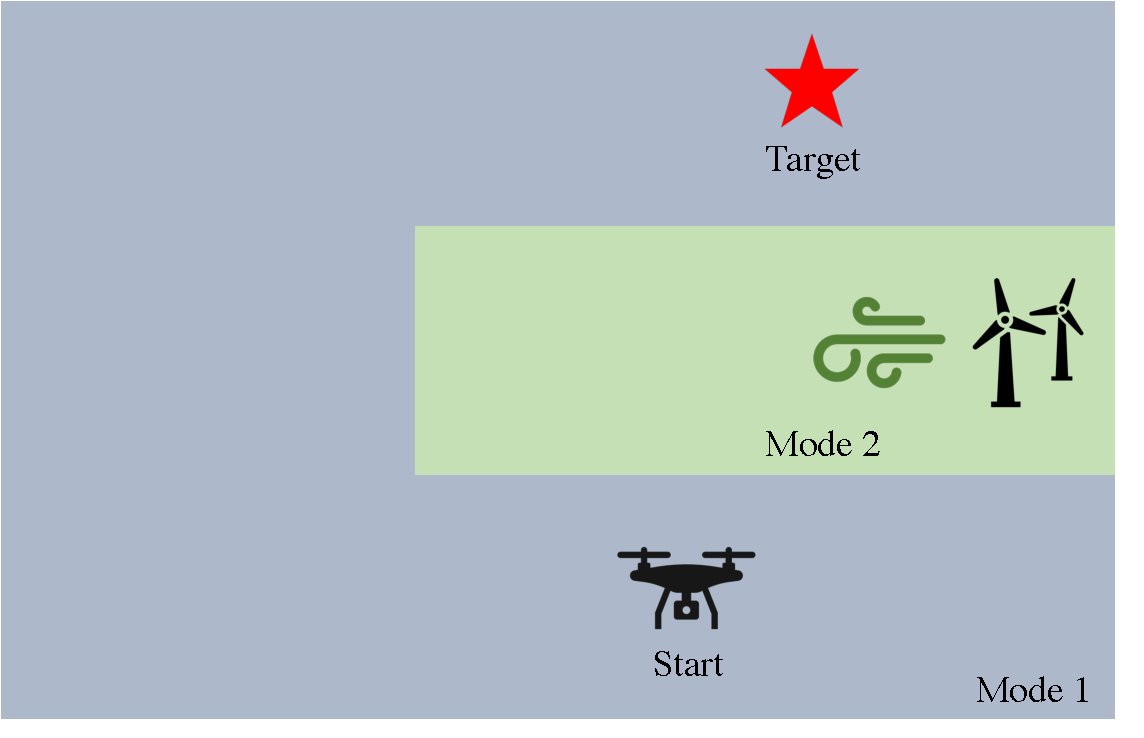
\includegraphics[width=0.85\textwidth]{../images/scenario-7-domain.pdf}
\end{center}
\end{frame}
\begin{frame}[label={sec:orgdf4a20d}]{}
\begin{center}
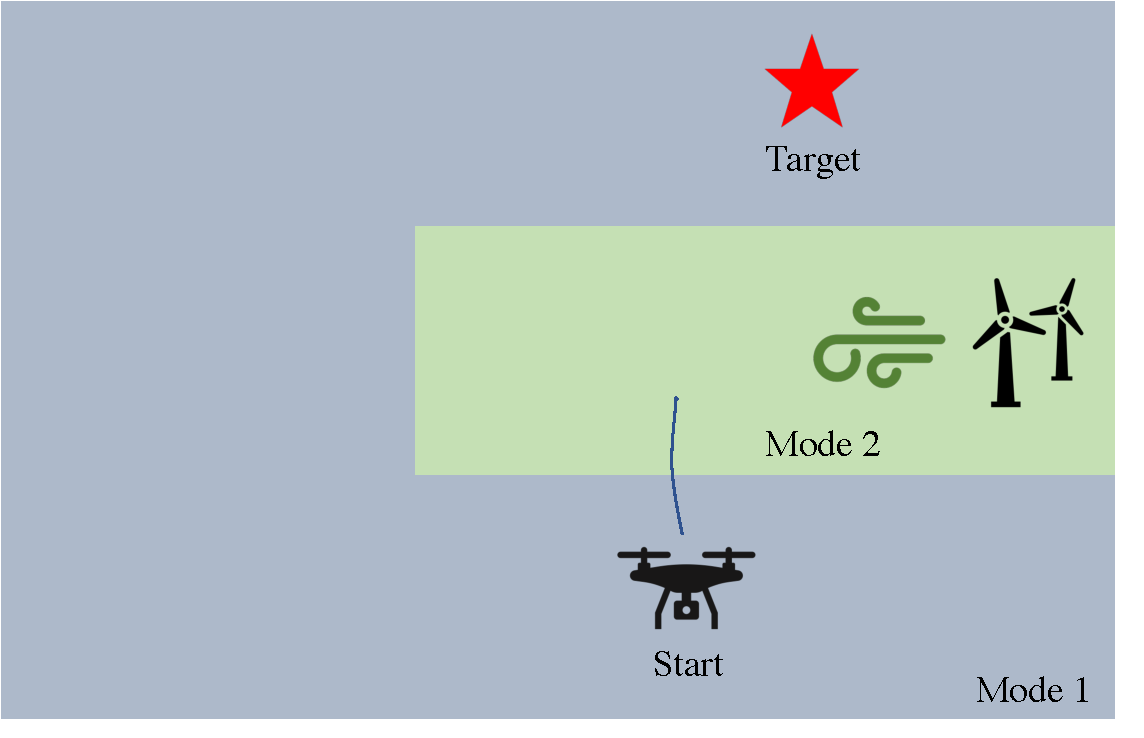
\includegraphics[width=0.85\textwidth]{../images/scenario-7-domain-crash-1.pdf}
\end{center}
\end{frame}
\begin{frame}[label={sec:org6307aa7}]{}
\begin{center}
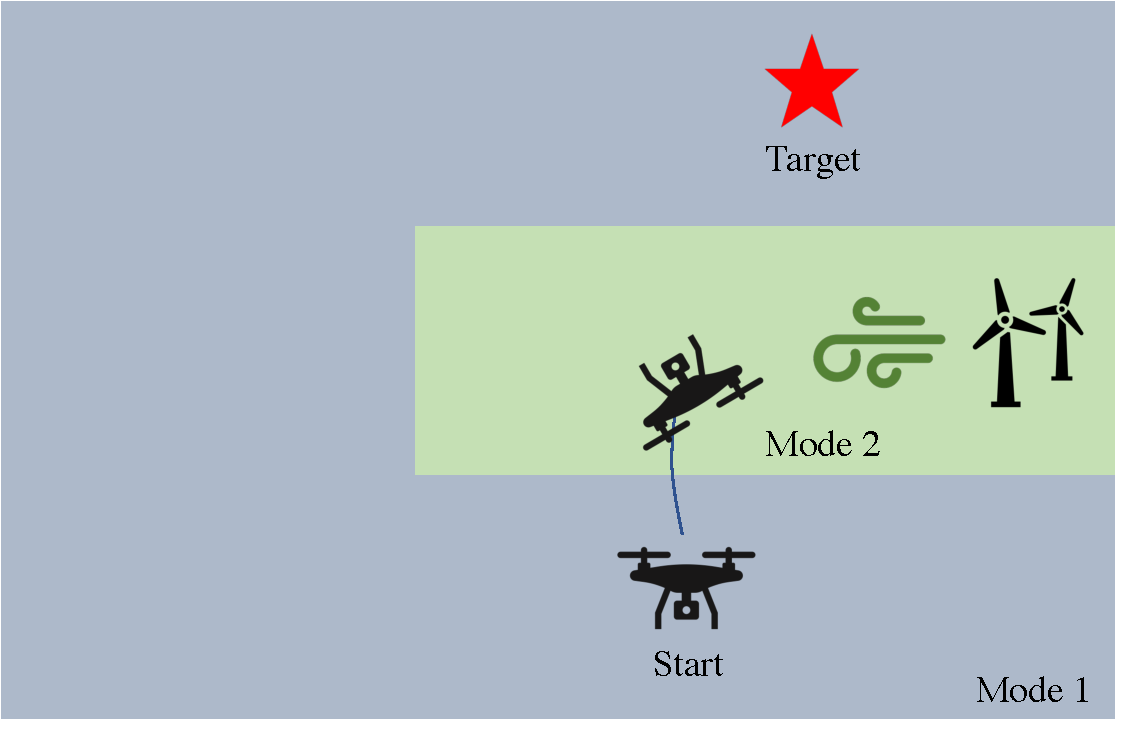
\includegraphics[width=0.85\textwidth]{../images/scenario-7-domain-crash-2.pdf}
\end{center}
\end{frame}
\begin{frame}[label={sec:org2d23175}]{}
\begin{center}
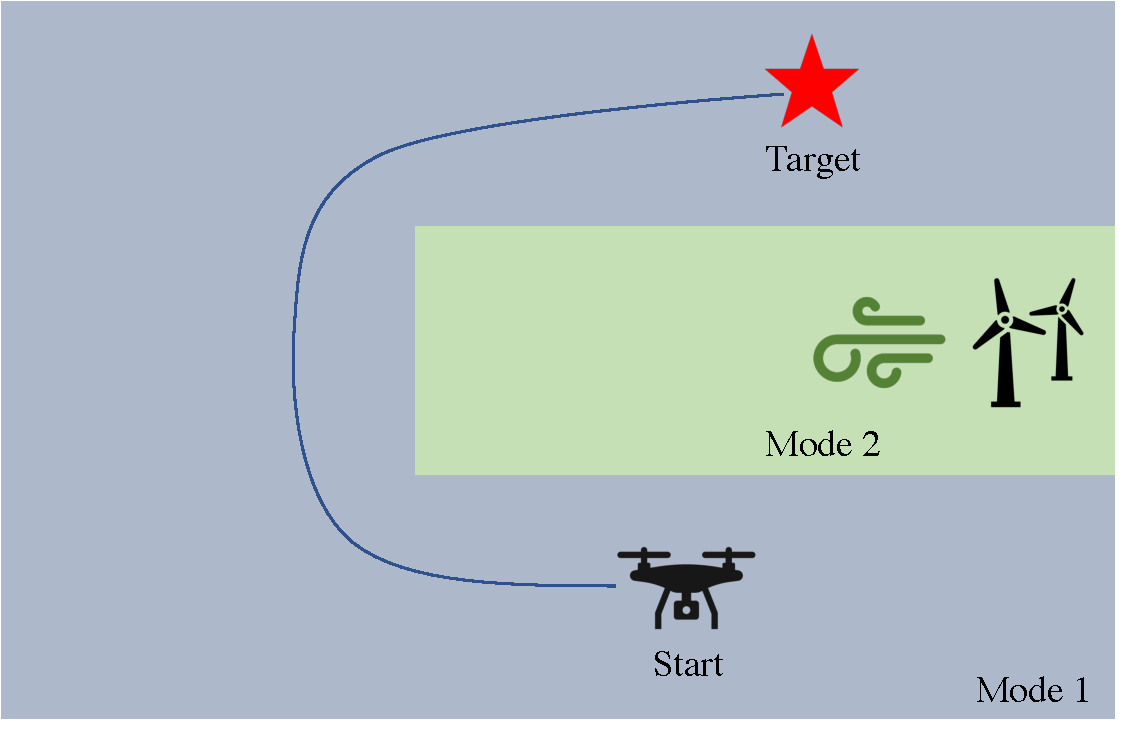
\includegraphics[width=0.85\textwidth]{../images/scenario-7-domain-success.pdf}
\end{center}
\end{frame}
\begin{frame}[label={sec:org0061d12}]{Goals}
\begin{description}[<+->]
\item[{Goal 1}] Navigate to the target state \(\targetState\)
\item[{Goal 2}] Remain in the operable, desired dynamics mode \(\desiredMode\)
\end{description}
\end{frame}

\begin{frame}[label={sec:org2099c2f}]{Mode remaining navigation problem}
\begin{myquote}
\begin{subequations}
\begin{align}
\min_{\policy \in \Pi} \quad
%&J_{\pi}(\state_0) \\
&\E \left[ \sum_{\timeInd=0}^{\TimeInd} \costFunc(\state_{\timeInd}, \pi(\state_{\timeInd}, \timeInd)) \mid \state_0=\state_0 \right] \\
%&\E \left[ \sum_{\timeInd=0}^{\TimeInd} \costFunc(\state_{\timeInd}, \pi(\state_{\timeInd}, \timeInd))
%\mid \state_0=\state \right] \\
\text{s.t.} \quad
&\onslide<4->{\state_{\timeInd+1} = \mode{\dynamicsFunc}(\state_\timeInd, \policy(\state_\timeInd, \timeInd)) + \mode{\bm\epsilon},
\quad \text{if } \modeVar(\state_{\timeInd}) = \modeInd \quad &\forall \timeInd \in \{0, \ldots, \TimeInd-1\}} \\
%&\text{\cref{eq-mode-remaining-def-explore}} \\
%&\onslide<2->{\dynamicsFunc(\state_{\timeInd}, \policy(\state_{\timeInd}, \timeInd)) \in \desiredStateDomain \quad &\forall \timeInd \in \{0, \ldots, \TimeInd-1\}} \\
&\onslide<5->{\modeVar(\state_{\timeInd}) = \desiredMode \quad &\forall \timeInd \in \{0, \ldots, \TimeInd-1\}} \\
&\onslide<2->{\state_{0} = \state_0} \\
&\onslide<3->{\state_\TimeInd = \targetState}
%\modeVar_{\timeInd} = \desiredMode \quad \forall \timeInd \in \mathbb{Z} \cap [0,\TimeInd] \\
%&\state_{\timeInd} \in \desiredStateDomain \quad \forall \timeInd \in \mathbb{Z} \cap [0,\TimeInd] \\
\end{align}
\end{subequations}
\end{myquote}
\end{frame}

\begin{frame}[label={sec:org4d7c6c6}]{Mode remaining navigation problem}
\begin{itemize}[<+->]
\item Dynamics and mode switching are \emph{unknown a priori}
\item So we cannot guarantee mode remaining behaviour\ldots{}
\begin{align}
&\modeVar(\state_{\timeInd}) = \desiredMode \quad &\forall \timeInd \in \{0, \ldots, \TimeInd-1\}
\end{align}
\item Solve using model-based reinforcement learning
\begin{itemize}
\item jointly learn dynamics modes and switching mechanism
\item relax mode remaining requirement
\begin{align}
\Pr( \forall \timeInd \in \{0,\ldots,\TimeInd \} : \modeVar(\state_{\timeInd}) &= \desiredMode,
\control_{\timeInd} \in \controlDomain) \geq 1 - \delta
\end{align}
\end{itemize}
\end{itemize}
\end{frame}

\begin{frame}[label={sec:orgee8e59e}]{Mode remaining model-based RL?}
\tikzstyle{startstop} = [rectangle, rounded corners, minimum width=2cm, minimum height=1cm,text centered, draw=black, fill=violet!30]
\tikzstyle{decision} = [diamond, rounded corners, minimum width=1cm, maximum height=1cm,text centered, draw=black, fill=violet!30]
%\tikzstyle{decision} = [diamond, minimum width=2cm, minimum height=0.5cm, text centered, draw=black, fill=violet!30]
\tikzstyle{arrow} = [thick,->,>=stealth]
% \begin{tikzpicture}[node distance=1.8cm, style={align=center}]]
\centering
\resizebox{0.7\textwidth}{!}{
\begin{tikzpicture}[every text node part/.style={align=center}, node distance=1.5cm]
\node (start) [startstop] {Learn dynamics model};
\node (trajopt) [startstop, below of=start, left of=start, xshift=-2cm] {Find trajectory to $\state_f$};
\node (constraints) [decision, below of=trajopt, yshift=-1cm] {$\delta-\text{mode}$\\ remaining?};
%# \node (constraints) [startstop, below of=trajopt] {$\delta-\text{mode remaining}$?};
\node (execute) [startstop, below of=constraints, yshift=-1cm] {Execute trajectory};
\node (explore) [startstop, right of=constraints, xshift=6cm] {$\delta-\text{mode exploration}$};

\draw [arrow] (start) -| (trajopt);
\draw [arrow] (trajopt) -- (constraints);
\draw [arrow] (constraints) -- node[anchor=east] {yes} (execute);
\draw [arrow] (constraints) -- node[anchor=south] {no} (explore);
\draw [arrow] (explore) |- node[anchor=west] {Experience} (start);
\end{tikzpicture}
}
\end{frame}


\begin{frame}[label={sec:orgd6f30a4}]{Contributions - Chapter 3}
\tikzstyle{startstop} = [rectangle, rounded corners, minimum width=2cm, minimum height=1cm,text centered, draw=black, fill=violet!30]
\tikzstyle{decision} = [diamond, rounded corners, minimum width=1cm, maximum height=1cm,text centered, draw=black, fill=violet!30]
%\tikzstyle{decision} = [diamond, minimum width=2cm, minimum height=0.5cm, text centered, draw=black, fill=violet!30]
\tikzstyle{arrow} = [thick,->,>=stealth]
% \begin{tikzpicture}[node distance=1.8cm, style={align=center}]]
\centering
\resizebox{0.7\textwidth}{!}{
\begin{tikzpicture}[every text node part/.style={align=center}, node distance=1.5cm]
\node (start) [startstop, fill=cyan!40] {Learn dynamics model};
\node (trajopt) [startstop, below of=start, left of=start, xshift=-2cm] {Find trajectory to $\state_f$};
\node (constraints) [decision, below of=trajopt, yshift=-1cm] {$\delta-\text{mode}$\\ remaining?};
%# \node (constraints) [startstop, below of=trajopt] {$\delta-\text{mode remaining}$?};
\node (execute) [startstop, below of=constraints, yshift=-1cm] {Execute trajectory};
\node (explore) [startstop, right of=constraints, xshift=6cm] {$\delta-\text{mode exploration}$};

\draw [arrow] (start) -| (trajopt);
\draw [arrow] (trajopt) -- (constraints);
\draw [arrow] (constraints) -- node[anchor=east] {yes} (execute);
\draw [arrow] (constraints) -- node[anchor=south] {no} (explore);
\draw [arrow] (explore) |- node[anchor=west] {Experience} (start);
\end{tikzpicture}
}
\end{frame}

\begin{frame}[label={sec:org1cc6742}]{Contributions - Chapter 4}
\tikzstyle{startstop} = [rectangle, rounded corners, minimum width=2cm, minimum height=1cm,text centered, draw=black, fill=violet!30]
\tikzstyle{decision} = [diamond, rounded corners, minimum width=1cm, maximum height=1cm,text centered, draw=black, fill=violet!30]
%\tikzstyle{decision} = [diamond, minimum width=2cm, minimum height=0.5cm, text centered, draw=black, fill=violet!30]
\tikzstyle{arrow} = [thick,->,>=stealth]
% \begin{tikzpicture}[node distance=1.8cm, style={align=center}]]
\centering
\resizebox{0.7\textwidth}{!}{
\begin{tikzpicture}[every text node part/.style={align=center}, node distance=1.5cm]
\node (start) [startstop] {Learn dynamics model};
\node (trajopt) [startstop, below of=start, left of=start, xshift=-2cm, fill=cyan!40] {Find trajectory to $\state_f$};
\node (constraints) [decision, below of=trajopt, yshift=-1cm, fill=cyan!40] {$\delta-\text{mode}$\\ remaining?};
%# \node (constraints) [startstop, below of=trajopt] {$\delta-\text{mode remaining}$?};
\node (execute) [startstop, below of=constraints, yshift=-1cm] {Execute trajectory};
\node (explore) [startstop, right of=constraints, xshift=6cm] {$\delta-\text{mode exploration}$};

\draw [arrow] (start) -| (trajopt);
\draw [arrow] (trajopt) -- (constraints);
\draw [arrow] (constraints) -- node[anchor=east] {yes} (execute);
\draw [arrow] (constraints) -- node[anchor=south] {no} (explore);
\draw [arrow] (explore) |- node[anchor=west] {Experience} (start);
\end{tikzpicture}
}
\end{frame}

\begin{frame}[label={sec:org1b72663}]{Contributions - Chapter 6}
\tikzstyle{startstop} = [rectangle, rounded corners, minimum width=2cm, minimum height=1cm,text centered, draw=black, fill=violet!30]
\tikzstyle{decision} = [diamond, rounded corners, minimum width=1cm, maximum height=1cm,text centered, draw=black, fill=violet!30]
%\tikzstyle{decision} = [diamond, minimum width=2cm, minimum height=0.5cm, text centered, draw=black, fill=violet!30]
\tikzstyle{arrow} = [thick,->,>=stealth]
% \begin{tikzpicture}[node distance=1.8cm, style={align=center}]]
\centering
\resizebox{0.7\textwidth}{!}{
\begin{tikzpicture}[every text node part/.style={align=center}, node distance=1.5cm]
\node (start) [startstop] {Learn dynamics model};
\node (trajopt) [startstop, below of=start, left of=start, xshift=-2cm] {Find trajectory to $\state_f$};
\node (constraints) [decision, below of=trajopt, yshift=-1cm] {$\delta-\text{mode}$\\ remaining?};
%# \node (constraints) [startstop, below of=trajopt] {$\delta-\text{mode remaining}$?};
\node (execute) [startstop, below of=constraints, yshift=-1cm] {Execute trajectory};
\node (explore) [startstop, right of=constraints, xshift=6cm, fill=cyan!40] {$\delta-\text{mode exploration}$};

\draw [arrow] (start) -| (trajopt);
\draw [arrow] (trajopt) -- (constraints);
\draw [arrow] (constraints) -- node[anchor=east] {yes} (execute);
\draw [arrow] (constraints) -- node[anchor=south] {no} (explore);
\draw [arrow] (explore) |- node[anchor=west] {Experience} (start);
\end{tikzpicture}
}
\end{frame}


\begin{frame}[label={sec:orgee4d5d7}]{ModeOpt iteration 0}
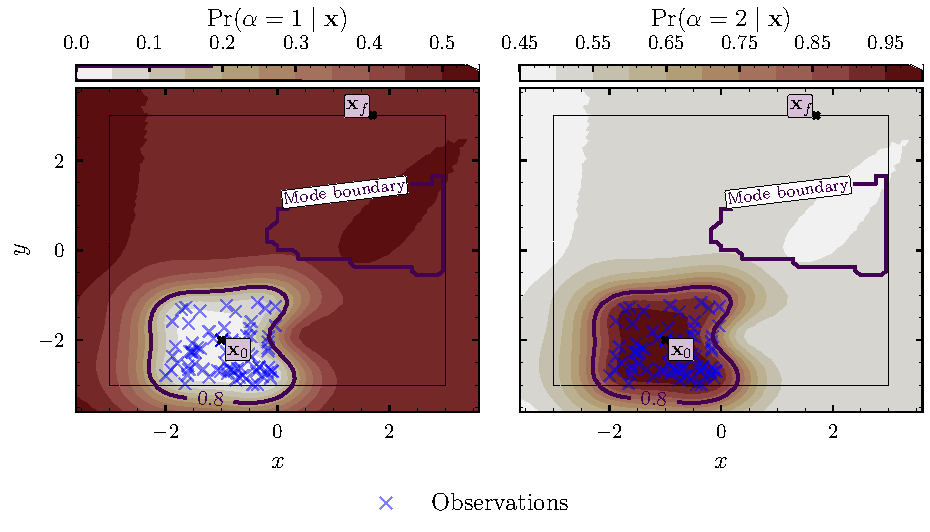
\includegraphics[width=0.8\textwidth]{../images/mode-opt/exploration/mvn-full-cov/data_over_mixing_probs_step_0_epoch_0.pdf}
\end{frame}
\begin{frame}[label={sec:org5a2b817}]{ModeOpt iteration 0}
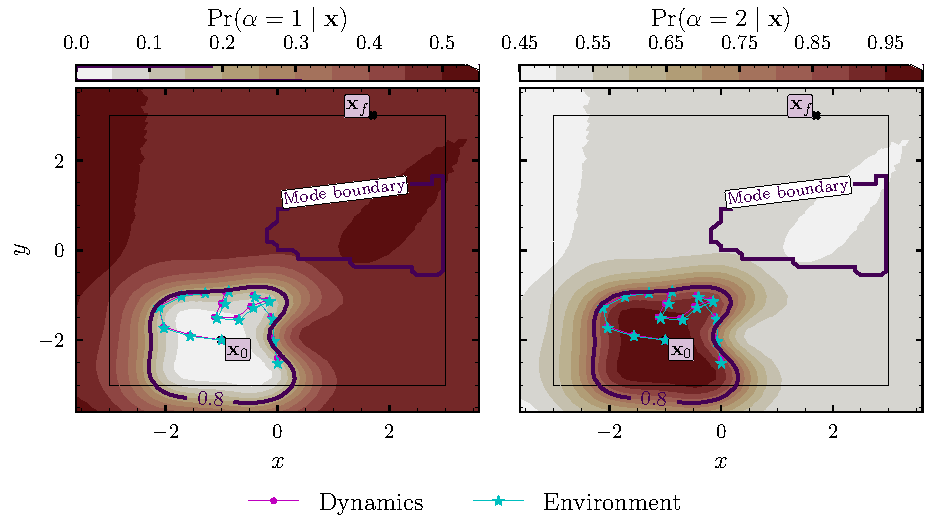
\includegraphics[width=0.8\textwidth]{../images/mode-opt/exploration/mvn-full-cov/trajectories_over_mixing_probs_step_1.pdf}
\end{frame}
\begin{frame}[label={sec:org2ef9566}]{ModeOpt iteration 0}
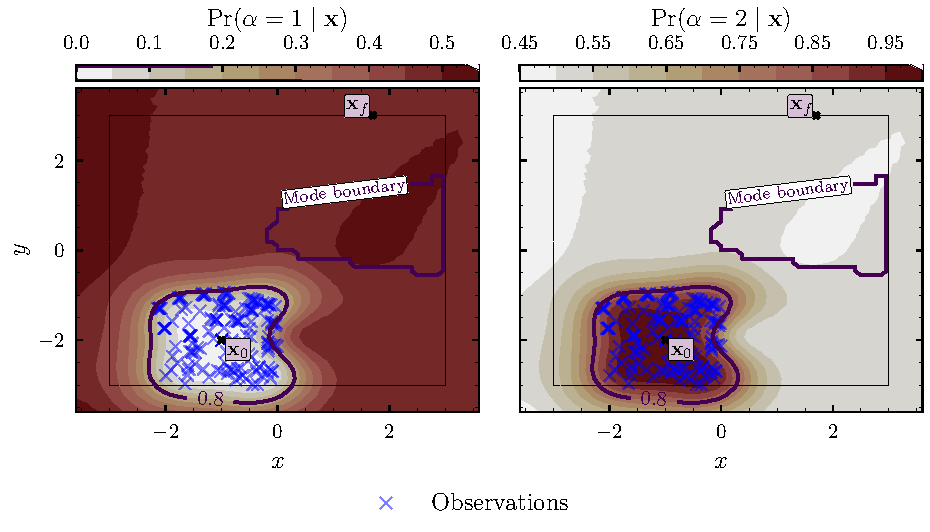
\includegraphics[width=0.8\textwidth]{../images/mode-opt/exploration/mvn-full-cov/data_over_mixing_probs_step_1_epoch_0.pdf}
\end{frame}
\begin{frame}[label={sec:org46c4490}]{ModeOpt iteration 1}
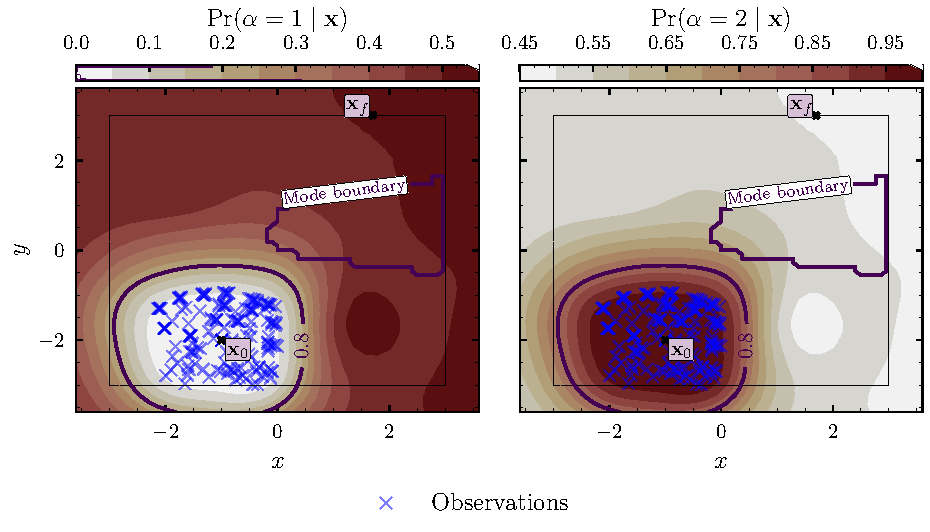
\includegraphics[width=0.8\textwidth]{../images/mode-opt/exploration/mvn-full-cov/data_over_mixing_probs_step_1_epoch_last.pdf}
\end{frame}
\begin{frame}[label={sec:orgc4a1653}]{ModeOpt iteration 1}
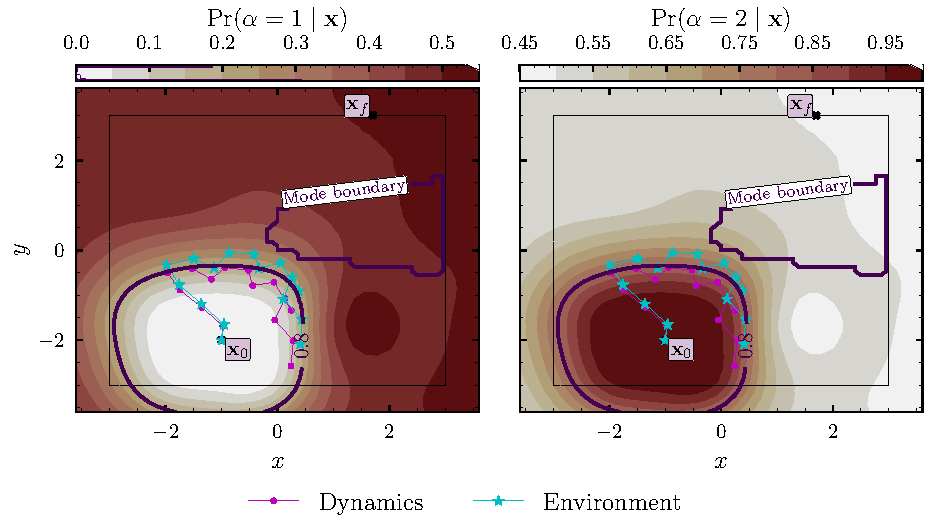
\includegraphics[width=0.8\textwidth]{../images/mode-opt/exploration/mvn-full-cov/trajectories_over_mixing_probs_step_2.pdf}
\end{frame}
\begin{frame}[label={sec:orgf513119}]{ModeOpt iteration 1}
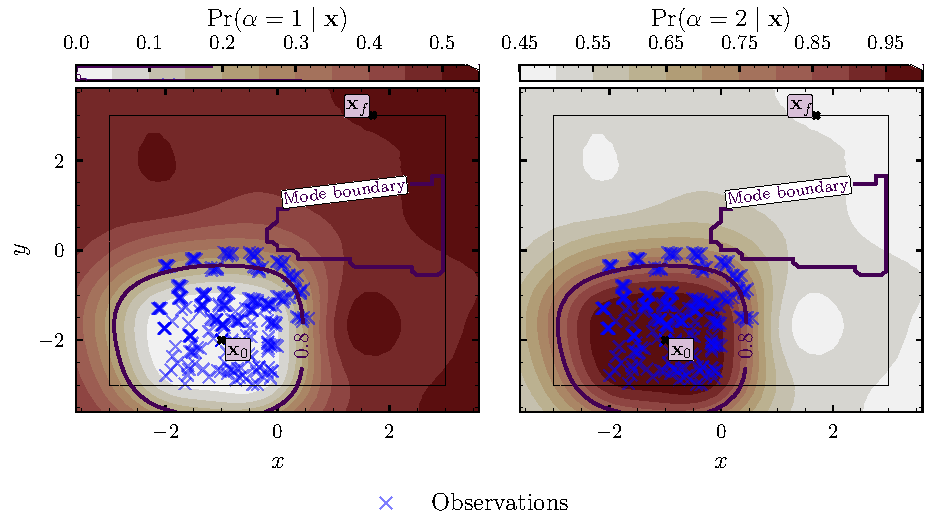
\includegraphics[width=0.8\textwidth]{../images/mode-opt/exploration/mvn-full-cov/data_over_mixing_probs_step_2_epoch_0.pdf}
\end{frame}
\begin{frame}[label={sec:orgc754d98}]{ModeOpt iteration 2}
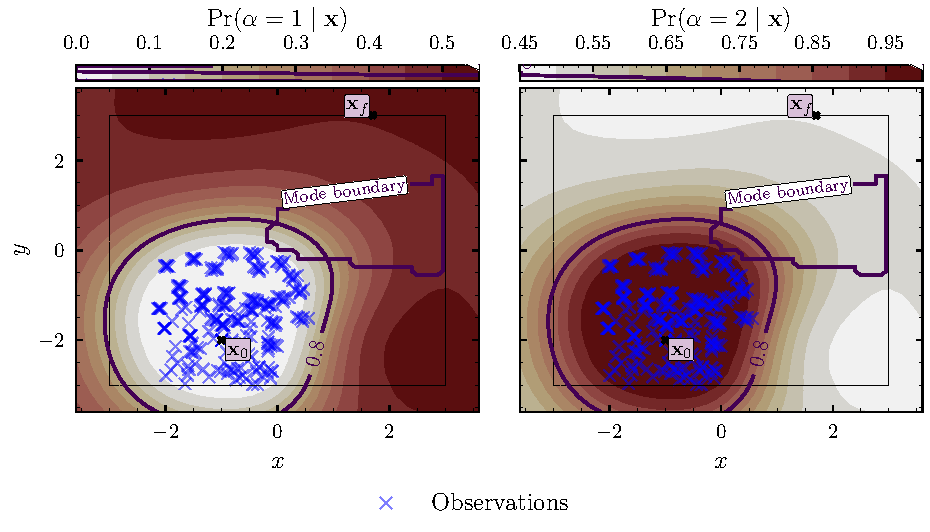
\includegraphics[width=0.8\textwidth]{../images/mode-opt/exploration/mvn-full-cov/data_over_mixing_probs_step_2_epoch_last.pdf}
\end{frame}
\begin{frame}[label={sec:org7569f0f}]{ModeOpt iteration 2}
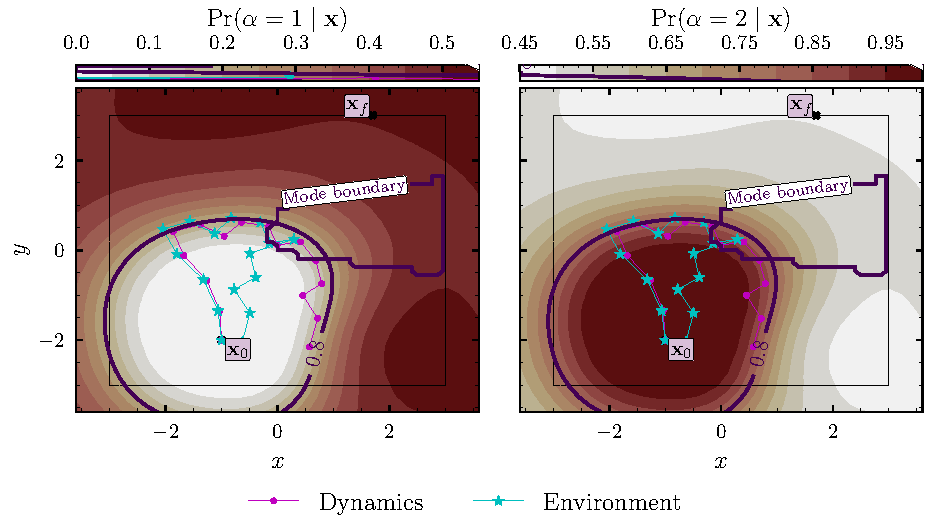
\includegraphics[width=0.8\textwidth]{../images/mode-opt/exploration/mvn-full-cov/trajectories_over_mixing_probs_step_3.pdf}
\end{frame}
\begin{frame}[label={sec:orgc7a019b}]{ModeOpt iteration 2}
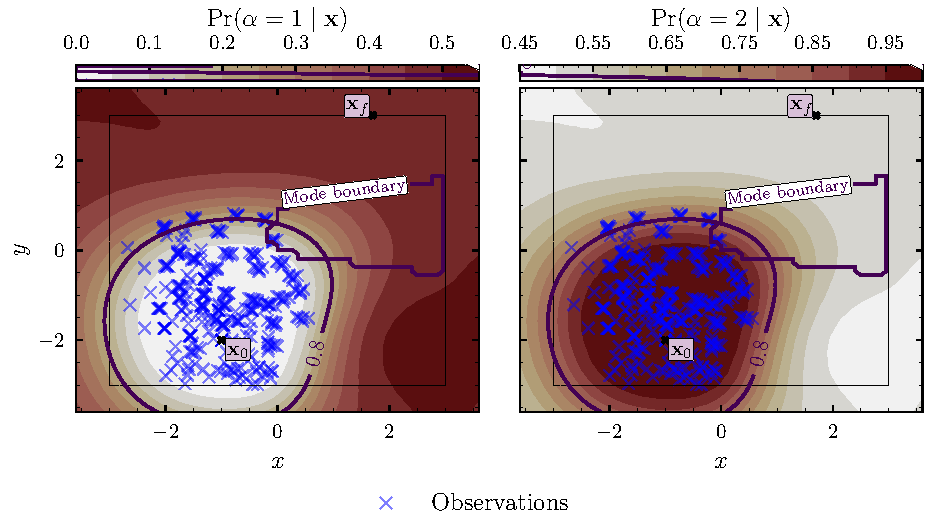
\includegraphics[width=0.8\textwidth]{../images/mode-opt/exploration/mvn-full-cov/data_over_mixing_probs_step_3_epoch_0.pdf}
\end{frame}
\begin{frame}[label={sec:org91235f7}]{ModeOpt iteration 3}
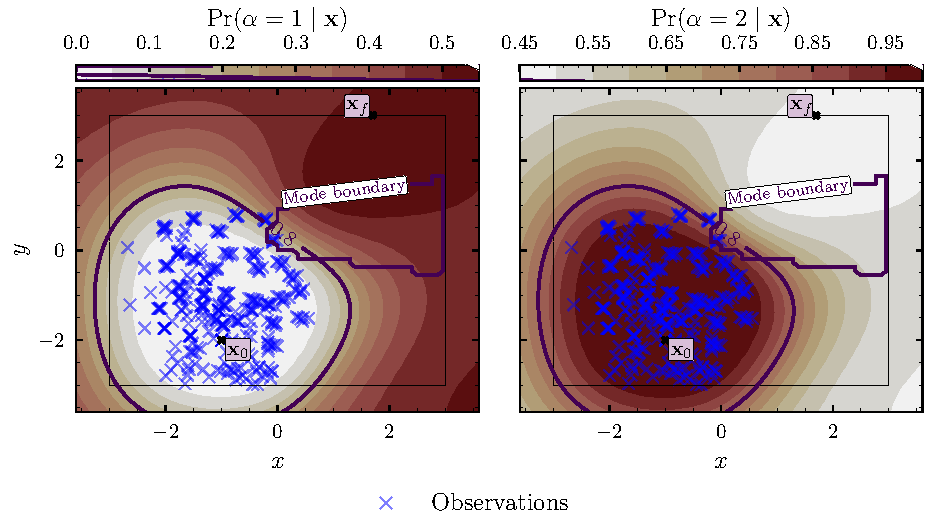
\includegraphics[width=0.8\textwidth]{../images/mode-opt/exploration/mvn-full-cov/data_over_mixing_probs_step_3_epoch_last.pdf}
\end{frame}

\begin{frame}[label={sec:org2b546d8}]{ModeOpt iteration 3}
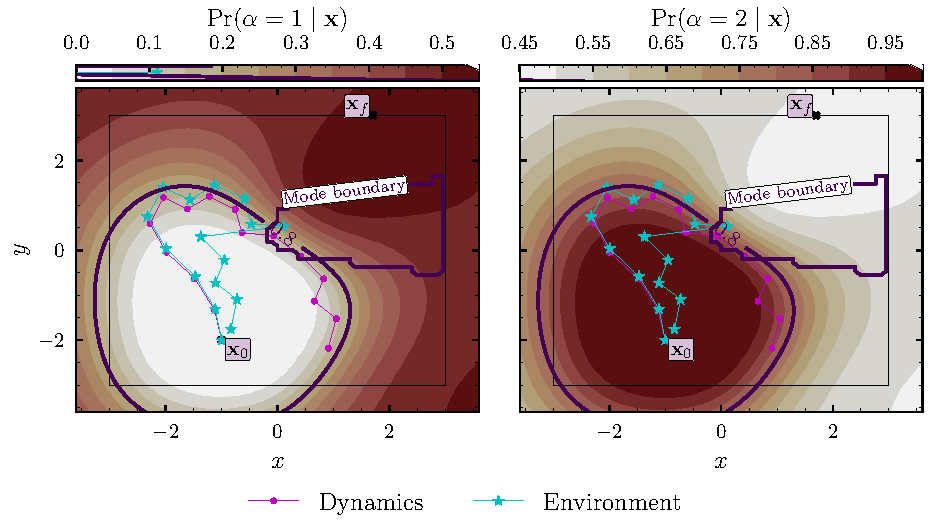
\includegraphics[width=0.8\textwidth]{../images/mode-opt/exploration/mvn-full-cov/trajectories_over_mixing_probs_step_4.pdf}
\end{frame}
\begin{frame}[label={sec:orgc0950a3}]{ModeOpt iteration 3}
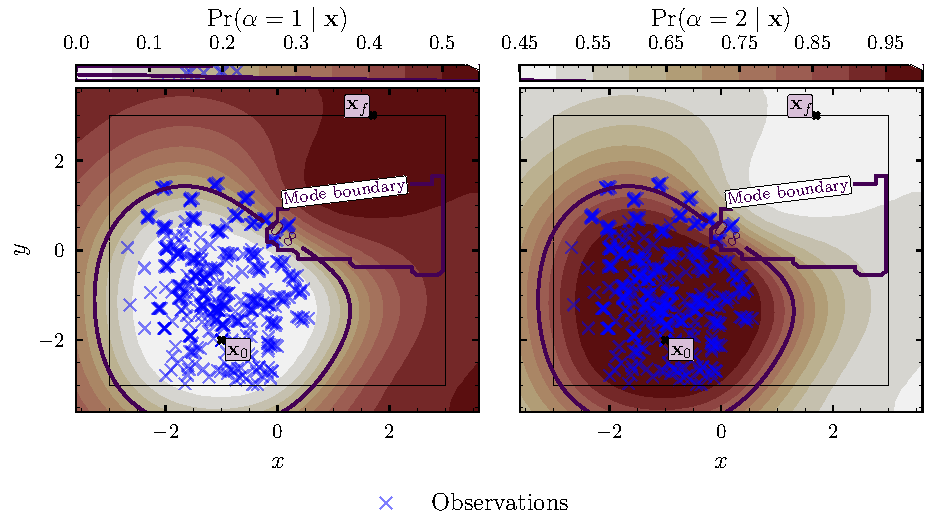
\includegraphics[width=0.8\textwidth]{../images/mode-opt/exploration/mvn-full-cov/data_over_mixing_probs_step_4_epoch_0.pdf}
\end{frame}
\begin{frame}[label={sec:orgaaed1d2}]{ModeOpt iteration 4}
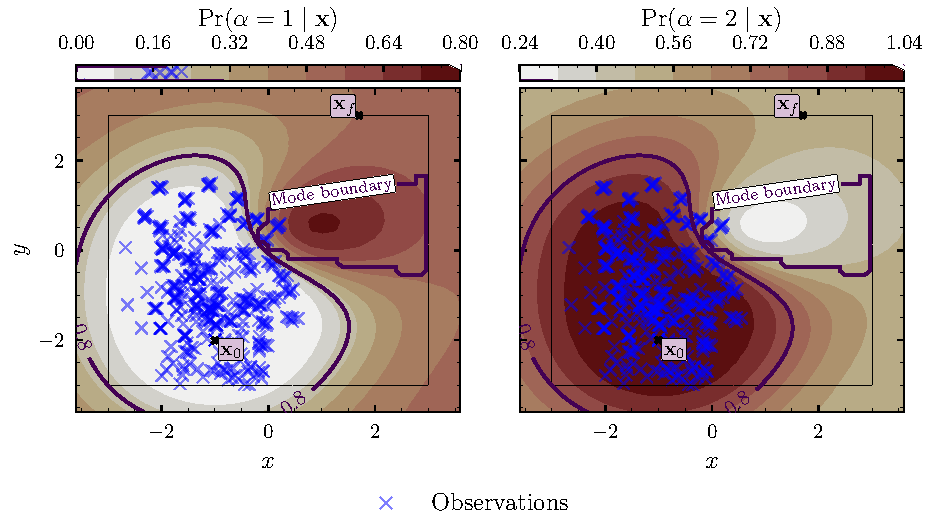
\includegraphics[width=0.8\textwidth]{../images/mode-opt/exploration/mvn-full-cov/data_over_mixing_probs_step_4_epoch_last.pdf}
\end{frame}
\begin{frame}[label={sec:org1219cab}]{ModeOpt iteration 4}
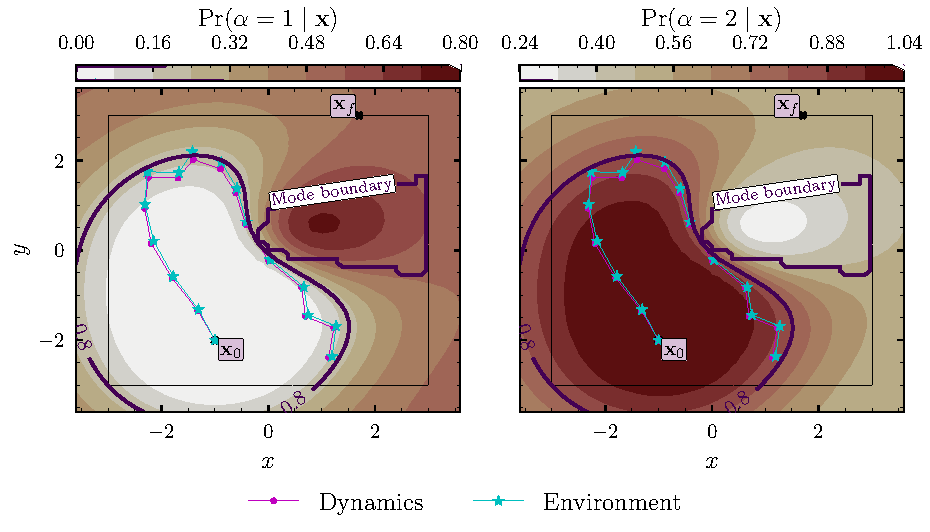
\includegraphics[width=0.8\textwidth]{../images/mode-opt/exploration/mvn-full-cov/trajectories_over_mixing_probs_step_5.pdf}
\end{frame}
\begin{frame}[label={sec:orgb03f1d2}]{ModeOpt iteration 4}
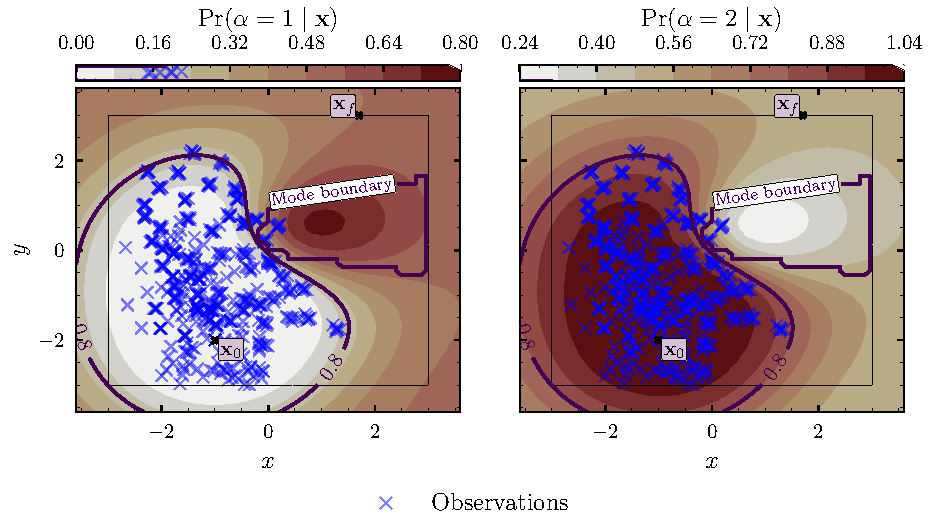
\includegraphics[width=0.8\textwidth]{../images/mode-opt/exploration/mvn-full-cov/data_over_mixing_probs_step_5_epoch_0.pdf}
\end{frame}
\begin{frame}[label={sec:org0224678}]{And so on, until}
\end{frame}
\begin{frame}[label={sec:org40fb659}]{And so on, until}
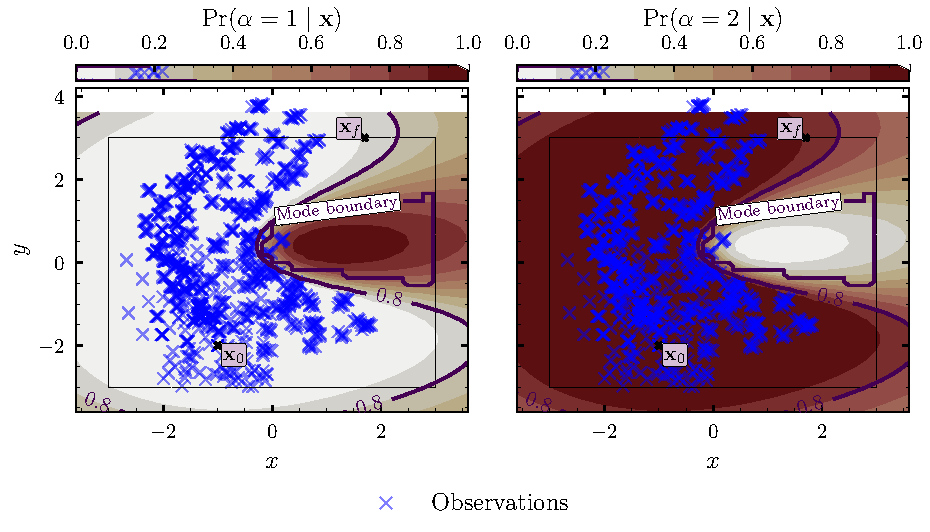
\includegraphics[width=0.8\textwidth]{../images/mode-opt/exploration/mvn-full-cov/data_over_mixing_probs_step_11_epoch_last.pdf}
\end{frame}


\begin{frame}[label={sec:orgc50440d},rightcolor=DarkPink,div=0.8\paperwidth]{Thanks for listening}
Questions?
\end{frame}


\begin{frame}[label={sec:orgdf511d8}]{Model learning - Mixture models?}
\begin{block}{MoE marginal likelihood}
\small
\begin{align} \label{eq-mixture-marginal-likelihood}
\moeEvidence = \prod_{\numData=1}^\NumData \sum_{\modeInd=1}^{\ModeInd}
\underbrace{\moeGatingPosterior}_{\text{gating network}}
\underbrace{\moeExpertPosterior}_{\text{expert } k},
\end{align}
\normalsize
\end{block}
\end{frame}
\begin{frame}[label={sec:orge5212fa}]{Model learning - Mixtures of Nonparametric Experts}
\begin{columns}
\begin{column}{0.3\columnwidth}
\newcommand{\gatingColor}{violet}
\newcommand{\expertColor}{orange}
\begin{figure}[t]
  \centering
    \begin{tikzpicture}[
      pre/.style={<-,shorten <=0.4pt,>=stealth',semithick},
      post/.style={->,shorten >=0.4pt,>=stealth',semithick}
      ]
      \node[const] (x) {$\singleInputK$};

      \node[latent, left=of x, yshift=-1.4cm] (f) {$\textcolor{\expertColor}{\mode{\latentFunc}(\allInputK)}$};

      \node[const, left=of f, xshift=0.4cm, \expertColor] (thetak) {$\textcolor{\expertColor}{\expertParamsK}$};

      \node[latent, below=of x, xshift=0.0cm] (a) {$\textcolor{\gatingColor}{\modeVarnk}$};

      \node[const, right=of a, xshift=-0.4cm, \gatingColor] (phik) {$\textcolor{\gatingColor}{\gatingParams}$};

      \node[obs, below=of f, yshift=0.4cm] (y) {$\allOutputK$};

      \node[const, left=of y, \expertColor] (sigmak) {$\textcolor{\expertColor}{\noiseVarK}$};

      \draw[post, \gatingColor] (a)--(y);
      \draw[post, \expertColor] (x)-|(f);
      \draw[post, \gatingColor] (x)--(a);
      \draw[post, \expertColor] (thetak)--(f);
      \draw[post, \gatingColor] (phik)--(a);
      \draw[post, \expertColor] (sigmak)|-(y);
      \draw[post, \expertColor] (f)--(y);

      \plate[color=\gatingColor] {} {(x) (yk) (a)} {$\textcolor{\gatingColor}{\NumData_{\modeInd}}$};
      \plate[color=\expertColor] {} {(x) (y) (f) (sigmak) (thetak) (a)} {$\ModeInd$};
    \end{tikzpicture}
    %}
\end{figure}
\end{column}

\begin{column}{0.65\columnwidth}
\newcommand{\gatingColor}{violet}
\newcommand{\expertColor}{orange}
%\small
\footnotesize
\begin{align*}  \label{eq-np-moe-marginal-likelihood-assign}
\moeEvidence  &= \sum_{\allModeVar} \textcolor{\gatingColor}{\npmoeGatingPosterior}
\left[ \prod_{\modeInd=1}^\ModeInd
\textcolor{\expertColor}{
\underbrace{
p\left(\{\singleOutput : \modeVarn=\modeInd \} \mid \{\singleInput : \modeVarn=\modeInd \}, \expertParamsK \right)}_{\text{expert } \modeInd}} \right]
\end{align*}
\normalsize
\begin{itemize}
\item Sum over exponentially many (\(\ModeInd^{\NumData}\)) sets of assignments
\begin{itemize}
\item \(\allModeVar = \{\modeVar_1, \ldots, \modeVar_\NumData \}\)
\end{itemize}
\end{itemize}
\end{column}
\end{columns}
\end{frame}
\begin{frame}[label={sec:org24680f8}]{Model learning - Identifiability}
\begin{columns}
\begin{column}{0.45\columnwidth}
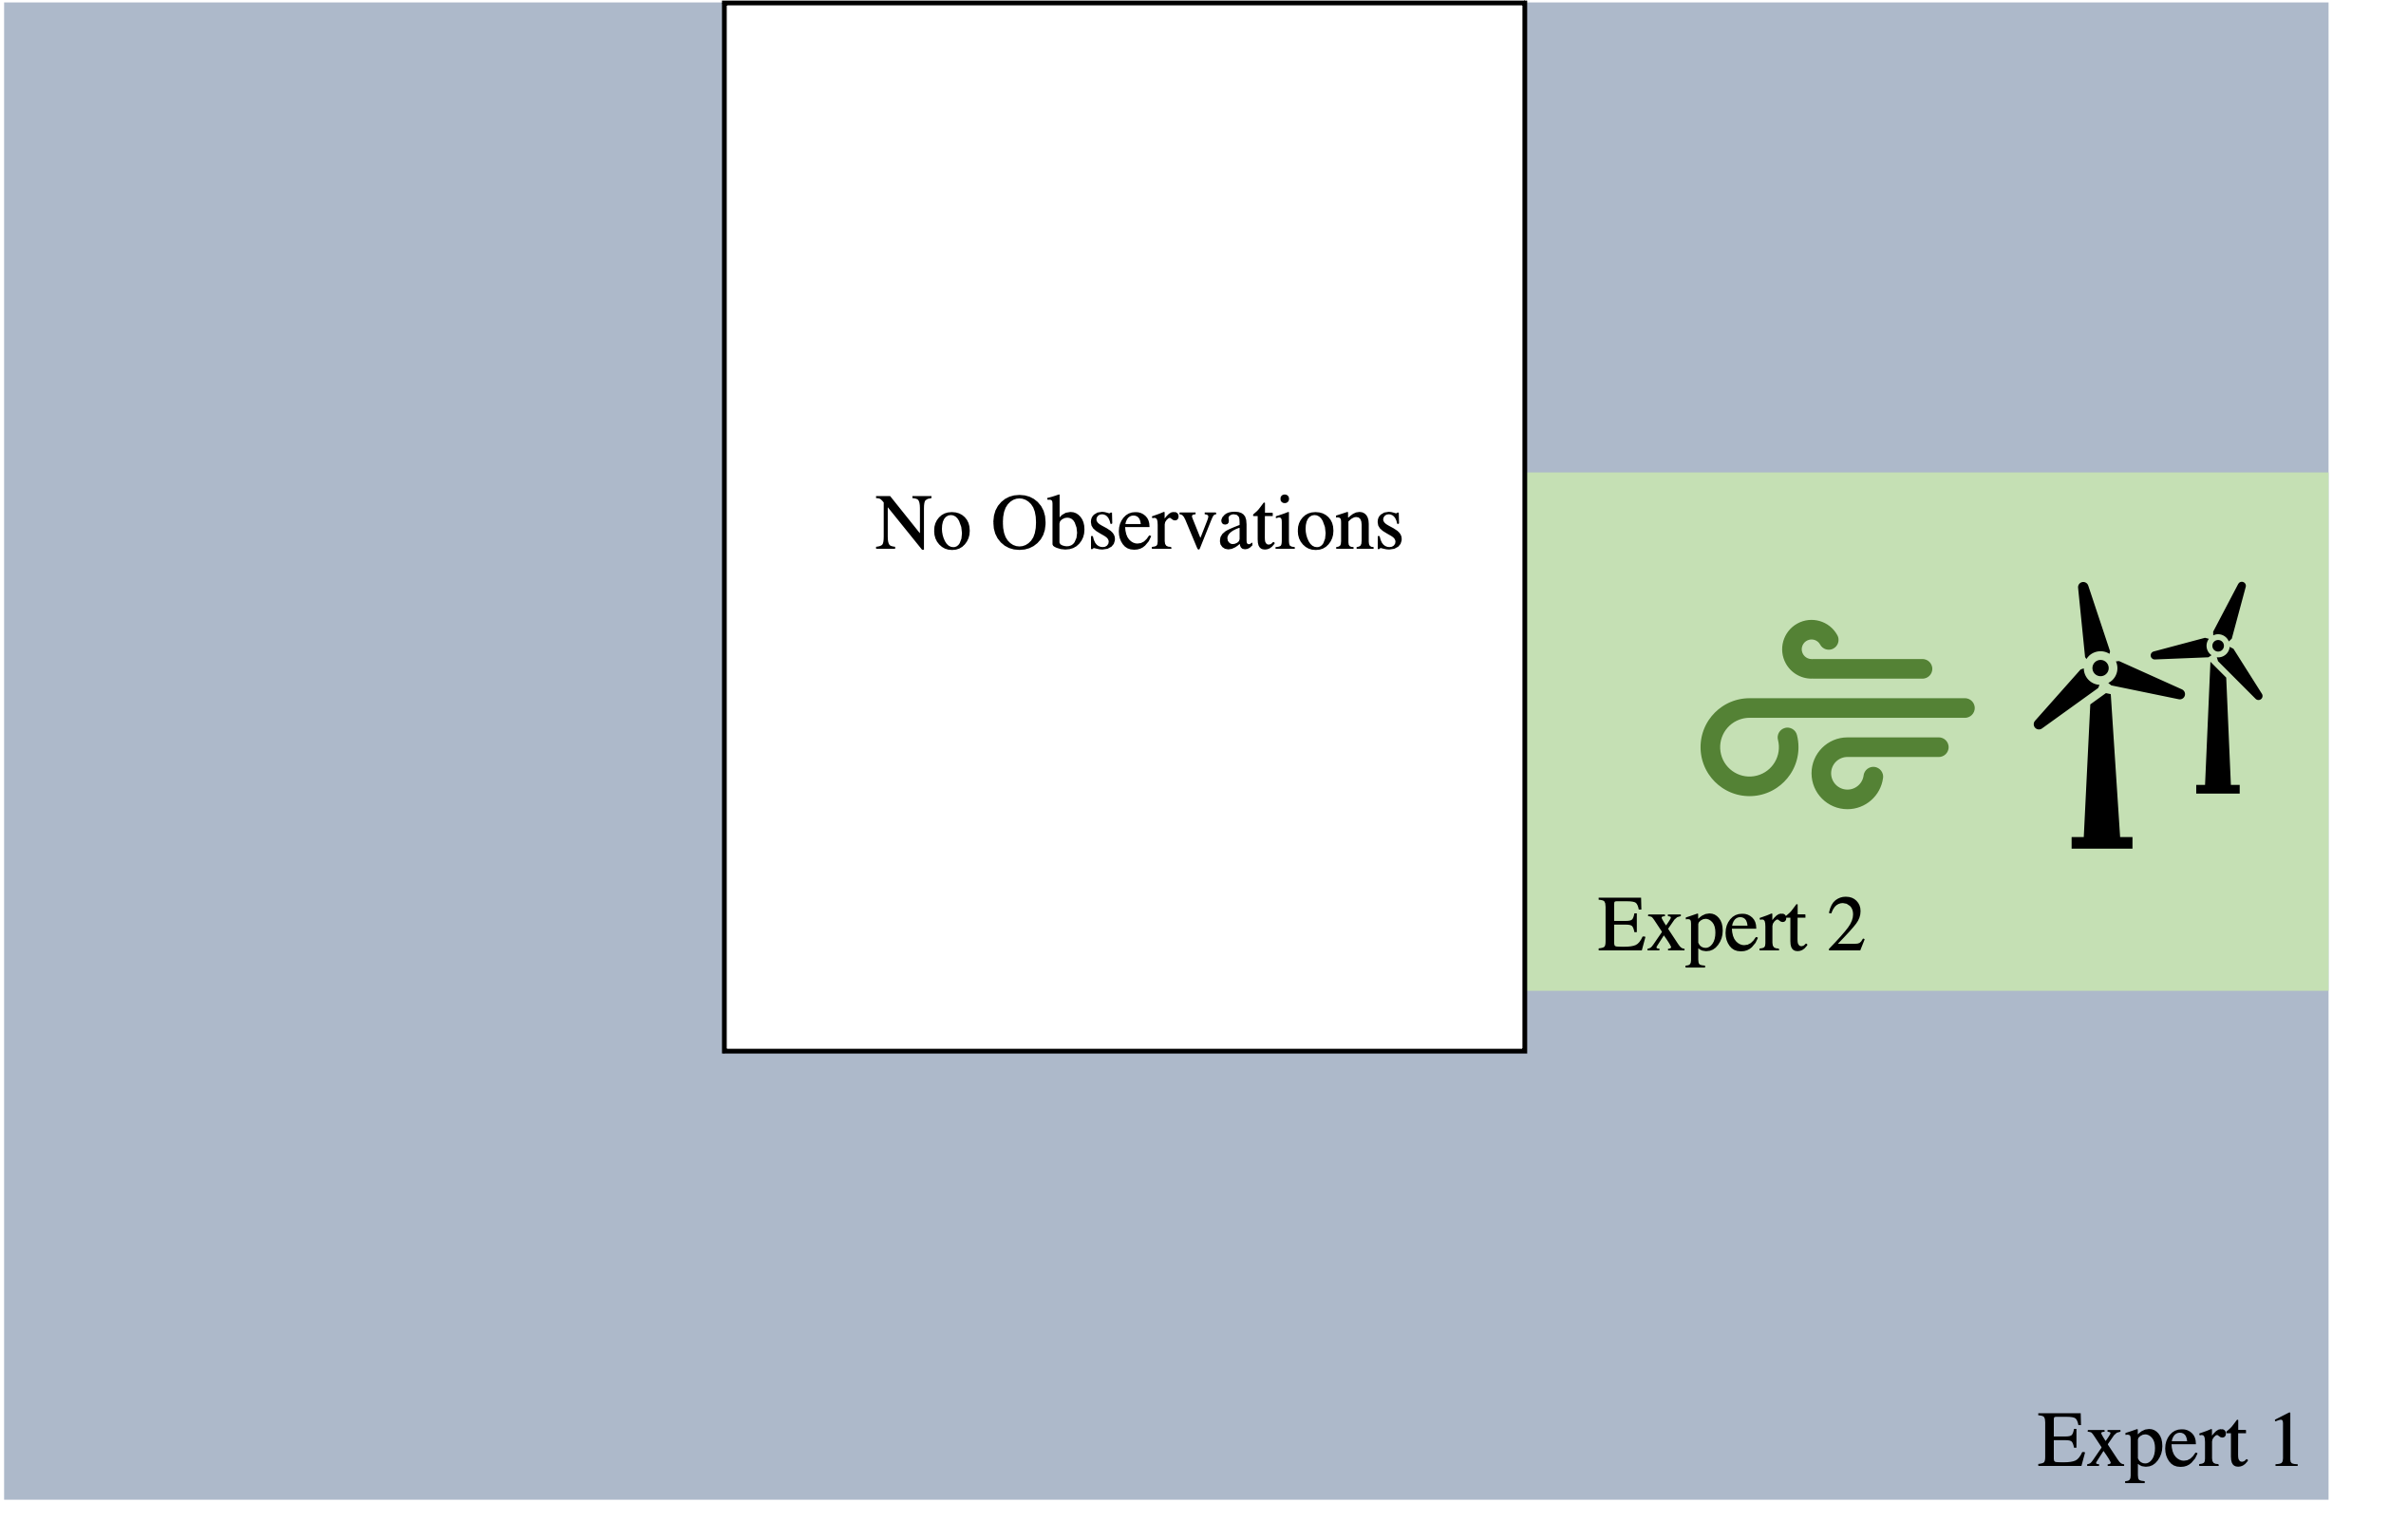
\includegraphics[width=\textwidth]{../images/quadcopter_domain_two_experts.png}
\end{column}
\begin{column}{0.45\columnwidth}
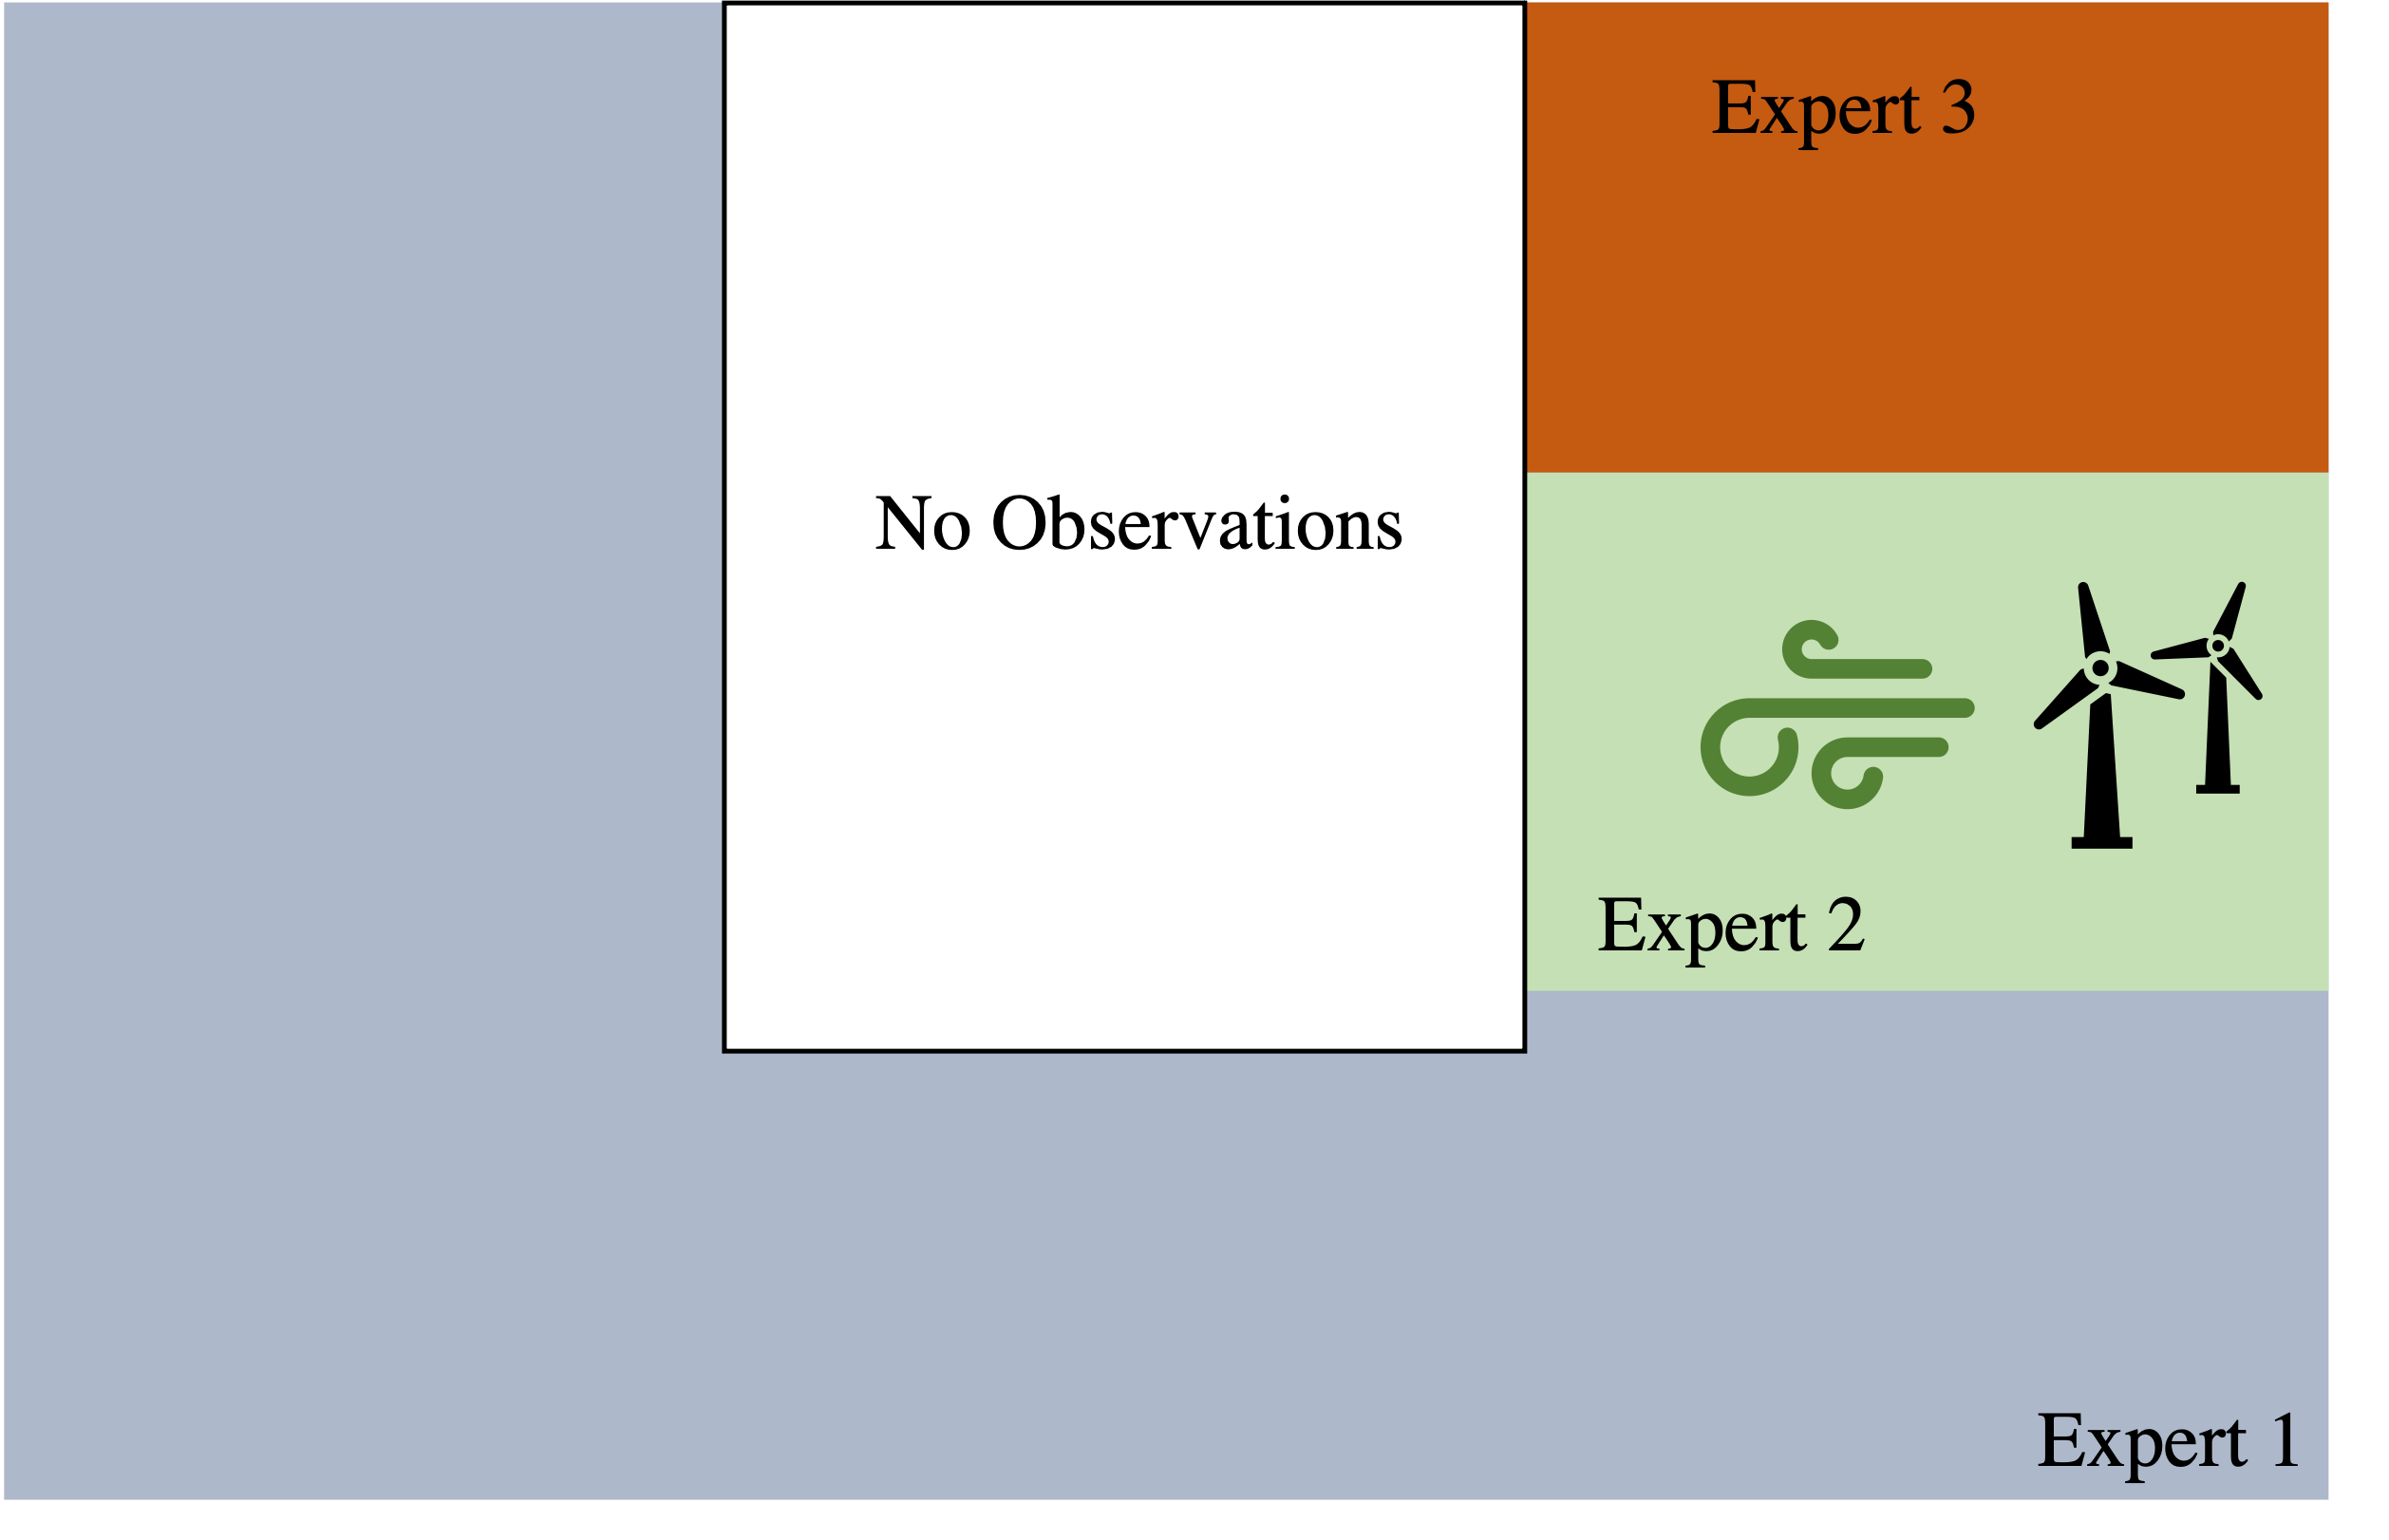
\includegraphics[width=\textwidth]{../images/quadcopter_domain_three_experts.png}
\end{column}
\end{columns}
\end{frame}

\begin{frame}[label={sec:orgf556ddc}]{Model learning - Mixtures of Nonparametric Experts}
\newcommand{\gatingColor}{violet}
\newcommand{\expertColor}{orange}
\begin{figure}[t]
  \centering
    \begin{minipage}[r]{0.49\textwidth}
%   \resizebox{0.8\columnwidth}{!}{
    \begin{tikzpicture}[
      pre/.style={<-,shorten <=0.4pt,>=stealth',semithick},
      post/.style={->,shorten >=0.4pt,>=stealth',semithick}
      ]
      \node[const] (x) {$\singleInputK$};

      \node[latent, left=of x, yshift=-1.4cm] (f) {$\textcolor{\expertColor}{\mode{\latentFunc}(\allInputK)}$};

      \node[const, left=of f, xshift=0.4cm, \expertColor] (thetak) {$\textcolor{\expertColor}{\expertParamsK}$};

      \node[latent, below=of x, xshift=0.0cm] (a) {$\textcolor{\gatingColor}{\modeVarnk}$};

      \node[const, right=of a, xshift=-0.4cm, \gatingColor] (phik) {$\textcolor{\gatingColor}{\gatingParams}$};

      \node[obs, below=of f, yshift=0.4cm] (y) {$\allOutputK$};

      \node[const, left=of y, \expertColor] (sigmak) {$\textcolor{\expertColor}{\noiseVarK}$};

      \draw[post, \gatingColor] (a)--(y);
      \draw[post, \expertColor] (x)-|(f);
      \draw[post, \gatingColor] (x)--(a);
      \draw[post, \expertColor] (thetak)--(f);
      \draw[post, \gatingColor] (phik)--(a);
      \draw[post, \expertColor] (sigmak)|-(y);
      \draw[post, \expertColor] (f)--(y);

      \plate[color=\gatingColor] {} {(x) (yk) (a)} {$\textcolor{\gatingColor}{\NumData_{\modeInd}}$};
      \plate[color=\expertColor] {} {(x) (y) (f) (sigmak) (thetak) (a)} {$\ModeInd$};
    \end{tikzpicture}
    %}
    \subcaption{}
\label{fig-graphical-model-npmoe}
\end{minipage}
    \begin{minipage}[r]{0.49\textwidth}
%   \resizebox{0.8\columnwidth}{!}{
    \begin{tikzpicture}[
      pre/.style={<-,shorten <=0.4pt,>=stealth',semithick},
      post/.style={->,shorten >=0.4pt,>=stealth',semithick}
      ]
      \node[const] (x) {$\singleInputK$};

      \node[latent, left=of x, yshift=-1.4cm] (f) {$\textcolor{\expertColor}{\mode{\latentFunc}(\allInputK)}$};
      \node[const, left=of f, xshift=0.4cm] (thetak) {$\textcolor{\expertColor}{\expertParamsK}$};

      \node[latent, below=of x, xshift=0.0cm] (a) {$\textcolor{\gatingColor}{\modeVarnk}$};
      \node[latent, right=of a, yshift=0.0cm] (h) {$\textcolor{\gatingColor}{\mode{\gatingFunc}(\allInput)}$};
      \node[const, right=of h, xshift=-0.4cm] (phik) {$\textcolor{\gatingColor}{\gatingParamsK}$};

      \node[obs, below=of f, yshift=0.4cm] (y) {$\allOutputK$};
      \node[const, left=of y] (sigmak) {$\textcolor{\expertColor}{\noiseVarK}$};

      \draw[post, \gatingColor] (a)--(y);
      \draw[post, \expertColor] (x)-|(f);
      \draw[post, \gatingColor] (x)-|(h);
      \draw[post, \gatingColor] (h)--(a);
      \draw[post, \expertColor] (thetak)--(f);
      \draw[post, \gatingColor] (phik)--(h);
      %\draw[post] (sigmak)|-(yk);
      \draw[post, \expertColor] (sigmak)|-(y);
      \draw[post, \expertColor] (f)--(y);

      \plate {} {(x) (yk) (a)} {$\textcolor{\gatingColor}{\NumData_{\modeInd}}$};
      %\plate {} {(zk) (uk) (f) (sigmak) (thetak) (yk)} {$K$};
      %\plate {} {(f) (sigmak) (thetak)} {$\ModeInd$};
      \plate[color=\gatingColor] {} {(h) (phik)} {$\textcolor{\gatingColor}{\ModeInd}$};
      \plate[color=\expertColor] {} {(x) (y) (f) (sigmak) (thetak)  (a)} {$\ModeInd$};
    \end{tikzpicture}
    %}
    \subcaption{}
\label{fig-graphical-model-gp-gating-network}
\end{minipage}
  %\caption{Graphical model where the output $\singleOutput$}
\label{fig-graphical-model-comparison}
\end{figure}
\end{frame}

\begin{frame}[label={sec:org6c05a00}]{Model learning - Identifiable Mixtures of Sparse Variational Gaussian Process Experts}
\newcommand{\gatingColor}{violet}
\newcommand{\expertColor}{orange}
\small
\begin{align}  \label{eq-np-moe-marginal-likelihood-assign}
\moeEvidence  &=
\sum_{\allModeVar}
\textcolor{\gatingColor}{\underbrace{\E_{\gatingPrior} \left[
\prod_{\numData=1}^{\NumData} \gatingLikelihood  \right]}_{\text{GP gating network}}}
\left[ \prod_{\modeInd=1}^\ModeInd
\textcolor{\expertColor}{
\underbrace{p\left(\{\singleOutput : \modeVarn=\modeInd \} \mid \{\singleInput : \modeVarn=\modeInd \}, \expertParamsK \right)}_{\text{expert } \modeInd}} \right]
\end{align}
\normalsize
\end{frame}

\begin{frame}[label={sec:org9aee6c4}]{Model learning - Parameterise the nonparametric model?}
\begin{itemize}[<+->]
\item Like a sparse GP parameterises a GP\ldots{}
\item GP prior where \(\allInputK = \{\singleInput : \modeVarK\}\)
\newcommand{\allInputKFull}{\ensuremath{\{\singleInput : \modeVarK\}}}
\begin{align} \label{eq-experts-inducing-prior}
\mode{\latentFunc}(\allInputK) &\sim \mathcal{N}\left( \expertMeanFunc(\allInputK), \expertCovFunc(\allInputK, \allInputK) \right)
\end{align}
\item Augment with inducing points
\begin{align} \label{eq-experts-inducing-prior}
\mode{\latentFunc}(\expertInducingInput)  &\sim  \mathcal{N}\left( \expertMeanFunc(\expertInducingInput),
\expertCovFunc(\expertInducingInput, \expertInducingInput) \right)
\end{align}
\item Approximate marginal likelihood
\begin{align} \label{eq-augmented-marginal-likelihood}
\evidence &\approx
\E_{\gatingsInducingPrior \expertsInducingPrior} \left[
\prod_{\numData=1}^{\NumData} \sum_{\modeInd=1}^{\ModeInd}
\singleGatingGivenInducing \singleExpertGivenInducing \right]
\end{align}
\end{itemize}
\end{frame}

\begin{frame}[label={sec:orgdf9ecdd}]{Model learning - Parameterise the nonparametric model?}
\begin{figure}[t]
  \centering
  \resizebox{0.8\columnwidth}{!}{
    \begin{tikzpicture}[
      pre/.style={<-,shorten <=0.4pt,>=stealth',semithick},
      post/.style={->,shorten >=0.4pt,>=stealth',semithick}
      ]
      \node[const] (x) {$\singleInput$};
      \node[latent, left=of x, yshift=-1.4cm] (f) {$\mode{\latentFunc}(\singleInput)$};
      %\node[latent, right=of x, yshift=-1.7cm] (h) {${h}^{(k)}_n$};
      \node[latent, right=of x, yshift=-1.4cm, xshift=0.5cm] (h) {$\mode{\gatingFunc}(\singleInput)$};

      \node[latent, left=of f, xshift=0.4cm, yshift=0.6cm] (uk) {$\expertInducingOutput$};
      \node[latent, right=of h, xshift=-0.4cm, yshift=0.6cm] (uh) {$\gatingInducingOutput$};
      \node[const, left=of uk, xshift=0.4cm] (zk) {$\expertInducingInput$};
      \node[const, right=of uh, xshift=-0.4cm] (zh) {$\gatingInducingInput$};

      \node[const, left=of f, xshift=0.4cm, yshift=-0.4cm] (thetak) {$\expertParamsK$};
      \node[const, right=of h, xshift=-0.4cm, yshift=-0.4cm] (phik) {$\gatingParamsK$};

      \node[const, below=of thetak, yshift=0.4cm] (sigmak) {$\noiseVarK$};

      \node[obs, right=of sigmak, yshift=0.cm, xshift=1.4cm] (y) {$\singleOutput$};
      %\node[latent, right=of y, below=of h] (a) {$\alpha_t$};
      \node[latent, right=of y, xshift=-0.4cm] (a) {$\modeVarn$};

      %\node[obs, right=of sigmak] (y) {$\Delta\mathbf{x}_{t}$};

      \factor[above=of a] {h-a} {left:Cat} {h} {a};

      \draw[post] (a)--(y);
      \draw[post] (x)-|(f);
      %\draw[post] (f)--(yk);
      \draw[post] (f)--(y);
      %\draw[post] (yk)--(y);
      %\draw[post] (h)--(a);
      \draw[post] (x)-|(h);
      \draw[post] (uk)--(f);
      \draw[post] (uh)--(h);
      \draw[post] (zk)--(uk);
      \draw[post] (zh)--(uh);
      \draw[post] (thetak)--(f);
      \draw[post] (phik)--(h);
      \draw[post] (sigmak)|-(y);

      \plate {} {(x) (y) (a) (f) (h)} {$\NumData$};
      %\plate {} {(zk) (uk) (f) (sigmak) (thetak) (yk)} {$K$};
      \plate {} {(zk) (uk) (f) (sigmak) (thetak)} {$\ModeInd$};
      \plate {} {(uh) (h) (phik)} {$\ModeInd$};
    \end{tikzpicture}
    }
\label{fig-graphical-model-sparse}
\end{figure}
\end{frame}
\end{document}
